% Options for packages loaded elsewhere
\PassOptionsToPackage{unicode}{hyperref}
\PassOptionsToPackage{hyphens}{url}
%
\documentclass[
  english,
  man]{apa6}
\usepackage{amsmath,amssymb}
\usepackage{lmodern}
\usepackage{ifxetex,ifluatex}
\ifnum 0\ifxetex 1\fi\ifluatex 1\fi=0 % if pdftex
  \usepackage[T1]{fontenc}
  \usepackage[utf8]{inputenc}
  \usepackage{textcomp} % provide euro and other symbols
\else % if luatex or xetex
  \usepackage{unicode-math}
  \defaultfontfeatures{Scale=MatchLowercase}
  \defaultfontfeatures[\rmfamily]{Ligatures=TeX,Scale=1}
\fi
% Use upquote if available, for straight quotes in verbatim environments
\IfFileExists{upquote.sty}{\usepackage{upquote}}{}
\IfFileExists{microtype.sty}{% use microtype if available
  \usepackage[]{microtype}
  \UseMicrotypeSet[protrusion]{basicmath} % disable protrusion for tt fonts
}{}
\makeatletter
\@ifundefined{KOMAClassName}{% if non-KOMA class
  \IfFileExists{parskip.sty}{%
    \usepackage{parskip}
  }{% else
    \setlength{\parindent}{0pt}
    \setlength{\parskip}{6pt plus 2pt minus 1pt}}
}{% if KOMA class
  \KOMAoptions{parskip=half}}
\makeatother
\usepackage{xcolor}
\IfFileExists{xurl.sty}{\usepackage{xurl}}{} % add URL line breaks if available
\IfFileExists{bookmark.sty}{\usepackage{bookmark}}{\usepackage{hyperref}}
\hypersetup{
  pdflang={en-EN},
  hidelinks,
  pdfcreator={LaTeX via pandoc}}
\urlstyle{same} % disable monospaced font for URLs
\usepackage{graphicx}
\makeatletter
\def\maxwidth{\ifdim\Gin@nat@width>\linewidth\linewidth\else\Gin@nat@width\fi}
\def\maxheight{\ifdim\Gin@nat@height>\textheight\textheight\else\Gin@nat@height\fi}
\makeatother
% Scale images if necessary, so that they will not overflow the page
% margins by default, and it is still possible to overwrite the defaults
% using explicit options in \includegraphics[width, height, ...]{}
\setkeys{Gin}{width=\maxwidth,height=\maxheight,keepaspectratio}
% Set default figure placement to htbp
\makeatletter
\def\fps@figure{htbp}
\makeatother
\setlength{\emergencystretch}{3em} % prevent overfull lines
\providecommand{\tightlist}{%
  \setlength{\itemsep}{0pt}\setlength{\parskip}{0pt}}
\setcounter{secnumdepth}{-\maxdimen} % remove section numbering
% Make \paragraph and \subparagraph free-standing
\ifx\paragraph\undefined\else
  \let\oldparagraph\paragraph
  \renewcommand{\paragraph}[1]{\oldparagraph{#1}\mbox{}}
\fi
\ifx\subparagraph\undefined\else
  \let\oldsubparagraph\subparagraph
  \renewcommand{\subparagraph}[1]{\oldsubparagraph{#1}\mbox{}}
\fi
% Manuscript styling
\usepackage{upgreek}
\captionsetup{font=singlespacing,justification=justified}

% Table formatting
\usepackage{longtable}
\usepackage{lscape}
% \usepackage[counterclockwise]{rotating}   % Landscape page setup for large tables
\usepackage{multirow}		% Table styling
\usepackage{tabularx}		% Control Column width
\usepackage[flushleft]{threeparttable}	% Allows for three part tables with a specified notes section
\usepackage{threeparttablex}            % Lets threeparttable work with longtable

% Create new environments so endfloat can handle them
% \newenvironment{ltable}
%   {\begin{landscape}\centering\begin{threeparttable}}
%   {\end{threeparttable}\end{landscape}}
\newenvironment{lltable}{\begin{landscape}\centering\begin{ThreePartTable}}{\end{ThreePartTable}\end{landscape}}

% Enables adjusting longtable caption width to table width
% Solution found at http://golatex.de/longtable-mit-caption-so-breit-wie-die-tabelle-t15767.html
\makeatletter
\newcommand\LastLTentrywidth{1em}
\newlength\longtablewidth
\setlength{\longtablewidth}{1in}
\newcommand{\getlongtablewidth}{\begingroup \ifcsname LT@\roman{LT@tables}\endcsname \global\longtablewidth=0pt \renewcommand{\LT@entry}[2]{\global\advance\longtablewidth by ##2\relax\gdef\LastLTentrywidth{##2}}\@nameuse{LT@\roman{LT@tables}} \fi \endgroup}

% \setlength{\parindent}{0.5in}
% \setlength{\parskip}{0pt plus 0pt minus 0pt}

% \usepackage{etoolbox}
\makeatletter
\patchcmd{\HyOrg@maketitle}
  {\section{\normalfont\normalsize\abstractname}}
  {\section*{\normalfont\normalsize\abstractname}}
  {}{\typeout{Failed to patch abstract.}}
\patchcmd{\HyOrg@maketitle}
  {\section{\protect\normalfont{\@title}}}
  {\section*{\protect\normalfont{\@title}}}
  {}{\typeout{Failed to patch title.}}
\makeatother
\shorttitle{SHORTTITLE}
\usepackage{csquotes}
\usepackage{float}
\usepackage{sectsty}
\ifxetex
  % Load polyglossia as late as possible: uses bidi with RTL langages (e.g. Hebrew, Arabic)
  \usepackage{polyglossia}
  \setmainlanguage[]{english}
\else
  \usepackage[main=english]{babel}
% get rid of language-specific shorthands (see #6817):
\let\LanguageShortHands\languageshorthands
\def\languageshorthands#1{}
\fi
\ifluatex
  \usepackage{selnolig}  % disable illegal ligatures
\fi

\author{\phantom{0}}
\date{}


\affiliation{\phantom{0}}

\begin{document}

\hypertarget{chapitre-5-les-tests-duxe9quivalence}{%
\section{Chapitre 5: les tests d'équivalence}\label{chapitre-5-les-tests-duxe9quivalence}}

\hypertarget{introduction-du-chapitre}{%
\subsection{Introduction du chapitre}\label{introduction-du-chapitre}}

Lorsqu'on applique un test d'hypothèse, l'hypothèse nulle la plus couramment définie est celle d'absence d'effet ou de différence entre les groupes (\textbf{nickerson\_null\_2000?}). Il arrive également parfois que les chercheurs définissent un intervalle de valeur comme hypothèse nulle, mais le plus souvent, cet intervalle est borné par la valeur 0 (\textbf{nickerson\_null\_2000?}), on parle alors d'hypothèse unilatérale. Avec cette stratégie, le rejet de l'hypothèse nulle constitue un soutien en faveur de la présence d'un effet non nul. Par contre, le non rejet de l'hypothèse nulle ne peut être interprété comme un soutien en faveur de l'absence d'effet. Il arrive pourtant fréquemment que des chercheurs fassent cette erreur d'interprétation. (\textbf{finch\_reporting\_2001?}), par exemple, ont reporté que parmis 150 articles publiés entre 1940 et 1999 dans le \emph{JAP} (\emph{Journal of Applied Psychology}), 38\% interprétaient un résultat non significatif comme une acceptation de l'hypothès nulle. Plus récemment, (\textbf{lakens\_equivalence\_2017?}) a noté que l'expression ``pas d'effet'' a été utilisée dans 108 articles publié dans \emph{Social Psychological and Personality Science} avant août 2016 et que dans presque tous les cas, c'était sur base du non rejet de l'hypothèse nulle que cette conclusion était tirée.

\begin{enumerate}
\def\labelenumi{(\arabic{enumi})}
\tightlist
\item
  A travers ce chapitre, notre premier objectif sera d'expliquer pourquoi le non-rejet de l'hypothèse nulle ne peut être assimilé à une acceptation de l'hypothèse nulle. (2) Nous expliquerons ensuite le principe des tests d'équivalence. (3) Nous concluerons ce chapitre sur un article dans lequel nous comparer les tests d'équivalence à une stratégie récement développée par Blume (le \(SGPV\)).
\end{enumerate}

\hypertarget{quand-veut-on-montrer-une-absence-deffet}{%
\subsection{Quand veut-on montrer une absence d'effet?}\label{quand-veut-on-montrer-une-absence-deffet}}

Il arrive que des chercheurs souhaitent obtenir un soutien en faveur d'une absence d'effet. A titre d'illustration, (\textbf{goertzen\_detecting\_2010?}) évoquent la situation où un chercheur désire écarter de potentielles covariables de leur analyse, en démontrant préalablement que ces variables ne sont pas corrélées à la variable dépendante. ESSAYER DE TROUVER ENCORE UN EXEMPLE. Or, on constate que très souvent,

\hypertarget{diffuxe9rence-entre-nrh0-et-ah0}{%
\subsection{(1) Différence entre NRH0 et AH0}\label{diffuxe9rence-entre-nrh0-et-ah0}}

Le premier problème avec la stratégie traditionnelle est le fait que conclure au non rejet de l'hypothèse nulle ne signifie pas que l'on puisse accepter l'hypothèse nulle. En pratique, même lorsqu'une vraie différence non nulle existe entre les moyennes de population, il arrive que l'on soit amenés à conclure au non rejet de l'hypothèse nulle. \emph{Dans le cas idéal où nous aurions un échantillon de taille suffisante pour détecter l'effet étudié avec suffisamment de puissance, ce taux resterait assez faible bien que non nul. Et dans la mesure où souvent, la puissance dans les études est assez basses, ce taux peut encore augmenter. (retrouver projet de recherche pour décrire un peu ça sur base de quelques références)}. Afin de l'illustrer, nous avons réalisé des simulations Monte Carlo pour un ensemble de 70 scénarios qui diffèrent en fonction de la taille des échantillons (\(n_j\)) et de la différence entre les moyennes des deux populations dont sont extraits les échantillons (\(\mu_1-\mu_2\); voir Table 1). Pour chaque scénario, à 5000 reprises, nous avons généré une paire d'échantillons, réalisé un test \(t\) de Student pour échantillons indépendants et extrait la \(p\)-valeur du test, de sorte à obtenir au final 5000 \(p\)-valeur par scénario. Les résultats qui apparaissent au sein de la table 1 correspondent, pour chaque scénario, à la proportion de \(p\)-valeurs \emph{supérieures} à .05, le risque alpha communément accepté par les chercheurs \footnote{Cette proportion est ce qu'on appelle communément $\beta$, le taux d'erreur de type II.} {[}référence?{]}. Etant donné que dans tous les scénarios envisagés, la différence entre les moyennes de population est non nulle, on souhaiterait sur le long terme conclure le plus souvent possible au rejet de l'hypothèse nulle. Dit autrement, on souhaiterait que \(\beta\) soit le plus faible possible. Pourtant, il s'avère très élevé pour certains scénarios. Par exemple, avec 10 sujets par groupes et une taille d'effet standardisée de .1, on conclut dans près de 95\% des cas au non rejet de l'hypothèse nulle. On peut constater qu'avec une telle taille d'effet, même avec 200 sujets par groupes, on est encore amenés à conclure au non rejet de l'hypothèse nulle plus de 8 fois sur 10.

Le deuxième problème avec l'approche traditionnelle est que la probabilité de détecter l'absence d'effet va diminuer non seulement (1) quand la taille des échantillons augmente, mais également (2) quand l'erreur (la variabilité des scores au sein de chaque groupe) va augmenter {[}Meyners, voir power point{]}. On se retrouve alors dans la situation paradoxale où la probabilité de démontrer l'absence d'effet augmente lorsque des petits échantillons sont associés à une grande erreur de mesure {[}Meyners{]}.

Un test a de bonnes propriétés asymptotiques si sa puissance augmente à mesure que la taille des échantillons grandit. Or, plus les échantillons sont grands, \emph{moins} il est probable de conclure au non rejet de l'hypothèse nulle (soit en l'occurence, ce que les chercheurs tentent de démontrer lorsqu'ils postulent en faveur d'une absence d'effet). Ils se retrouvent alors dans une situation paradoxale où plus l'échantillon est grand, moins ils ont de chance de démontrer ce qu'ils veulent démontrer.

\begin{center}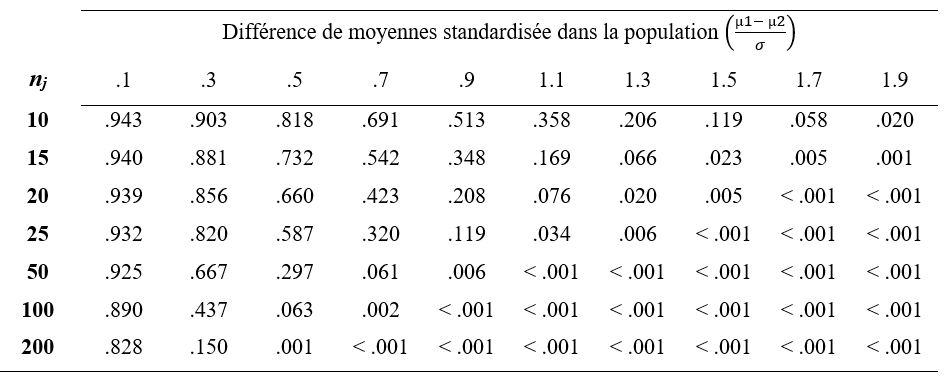
\includegraphics[width=3.15in]{C:/Users/Admin/OneDrive/Documents/Github projects/thesis/Chapitre 5/Illustration/Illustration} \end{center}

Table: Proportion de \(p\)-valeurs supérieures à .05 (\(\beta\)) en fonction de \(n_j\) et \(\mu_1-\mu_2\).
\emph{Note}. Pour chaque scénario, les deux échantillons sont toujours de même taille (\(n_j=n_1=n_2\)) et sont extraits de populations se distribuant normalement et ayant la même variance (\(\sigma_1=\sigma_2=\sigma\)). La moyenne de la première population (\(\mu_1\)) vaut systématiquement 0, et celle de la deuxième population (\(\mu_2\)) varie de sorte à obtenir la différence de moyenne \(\mu_1-\mu_2\) désirée. Par ailleurs, \(\sigma\) vaut systématiquement 1, si bien que la différence de moyenne brute est égale au \(\delta\) de Cohen.

moderate. With a sample size of N ¼ 10, approximately 75\% of sample correlation values (in absolute value) exceed r ¼ :1, 40\% exceed r ¼ :3, and even 15\% exceed r ¼ :5. With larger sample sizes there is still substantial variability in correlation coefficients. With a sample size of N ¼ 20, approximately 40\% of sample correlation values exceed r ¼ :2, and 20\% exceed r ¼ :3. Even with a sample size of N ¼ 100, more than 30\% of sample correlation values exceed r ¼ :1.

-Au mieux, le non rejet de l'hypothèse nulle nous montre que les données ne sont pas incompatibles avec l'hypothèse nulle, mais cela ne veut en aucun cas dire qu'elles ne sont compatibles avec aucune autres hypothèse!

\hypertarget{principe-du-test-duxe9quivalence}{%
\subsection{Principe du test d'équivalence}\label{principe-du-test-duxe9quivalence}}

\hypertarget{morceau-qui-servira-peut-uxeatre-ou-pas}{%
\subsection{Morceau qui servira peut-être (ou pas)}\label{morceau-qui-servira-peut-uxeatre-ou-pas}}

D'après (\textbf{lakens\_practical\_2021?}), un test d'hypothèse (selon l'approche de Nayman-Pearson) vaut la peine à 2 conditions:\\
1) que l'hypothèse nulle soit assez plausible pour que son rejet puisse surprendre au moins certains;\\
2) le chercheur veut appliquer une procédure méthodol qui l'autorise à prendre des décisions quant à la manière d'agir, tout en contrôlant le taux d'erreur. Agir peut vouloir dire: adopter un traitement, une politique, une intervention, ou abandonner un domaine de rechercher, modifier une manipulation, ou de faire un certain type de déclaration ou revendication.\\
*One of the most widely suggested improvements of the use of p values is to replace null-ypothesis tests (where the goal is to reject ann effect of exactly 0) with tests of range predictions (where the goal is to reject effects that fall outside of the range of effects that is predicted or considered practically important) (\textbf{lakens\_practical\_2021?}).

Un autre argument en défaveur de la p-valeur est la tendance des chercheurs à interpréter un effet NS comme l'acceptation de l'hypothèse nulle (Schmidt, 1996, cité par Harris, 1997). Une fois encore, l'usage des tailles d'effet peut aider à cette fin, non pas en ``remplaçant'' les tests d'hypothèses, mais en les complétant. --\textgreater{} Tests d'équivalence.

\begin{center}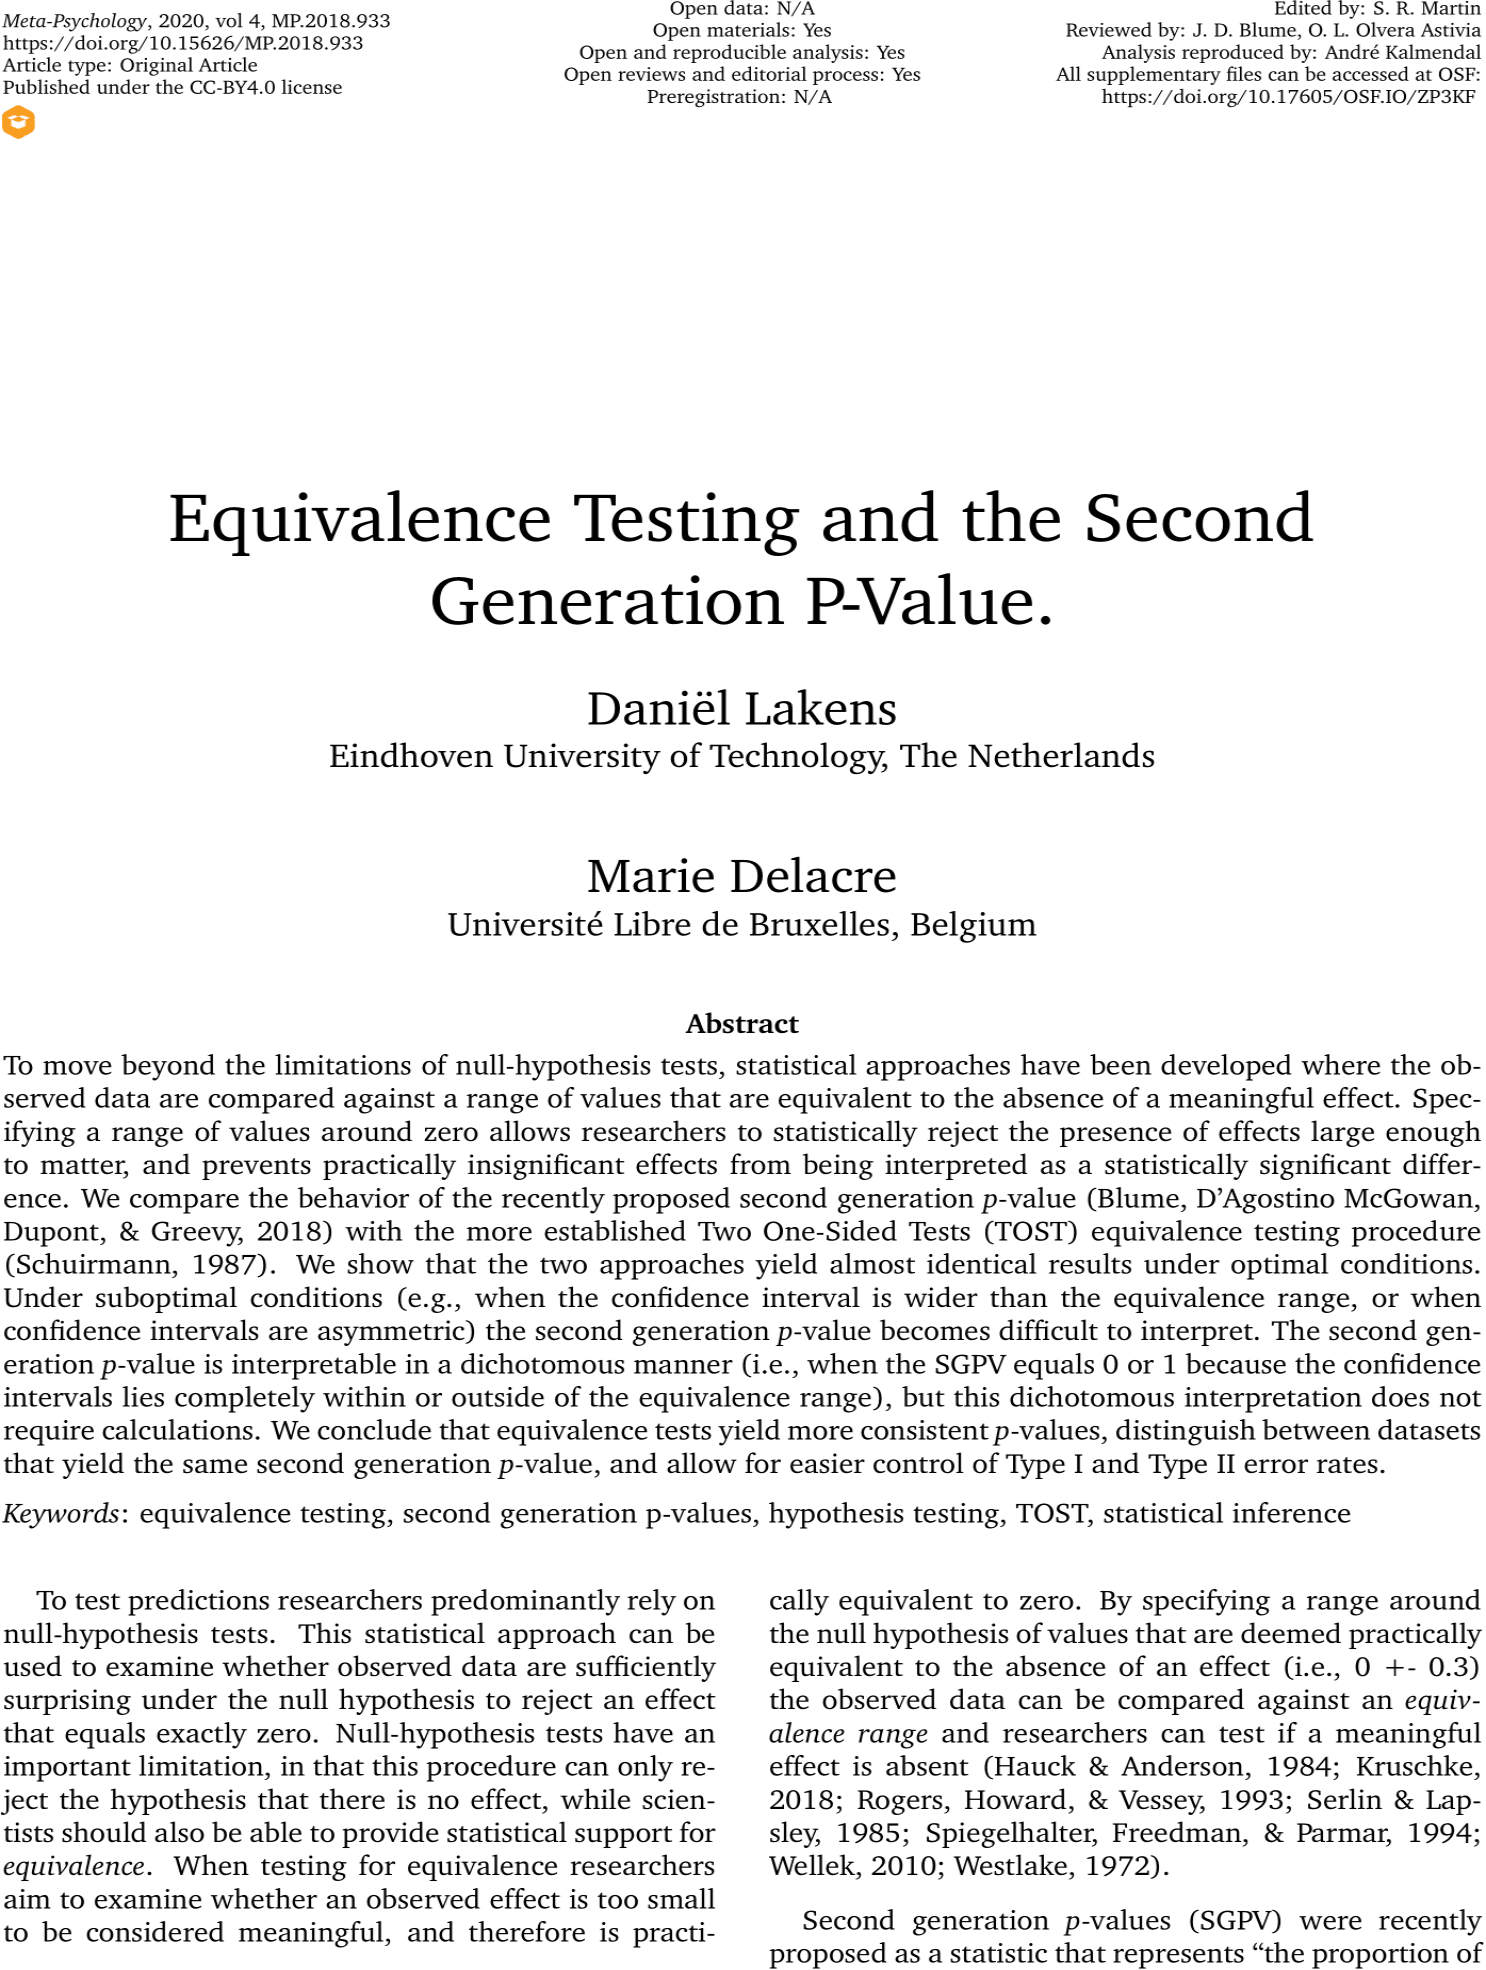
\includegraphics[width=0.92\linewidth]{C:/Users/Admin/OneDrive/Documents/Github projects/thesis/Chapitre 5/Chapitre 5-1} \end{center}

\begin{center}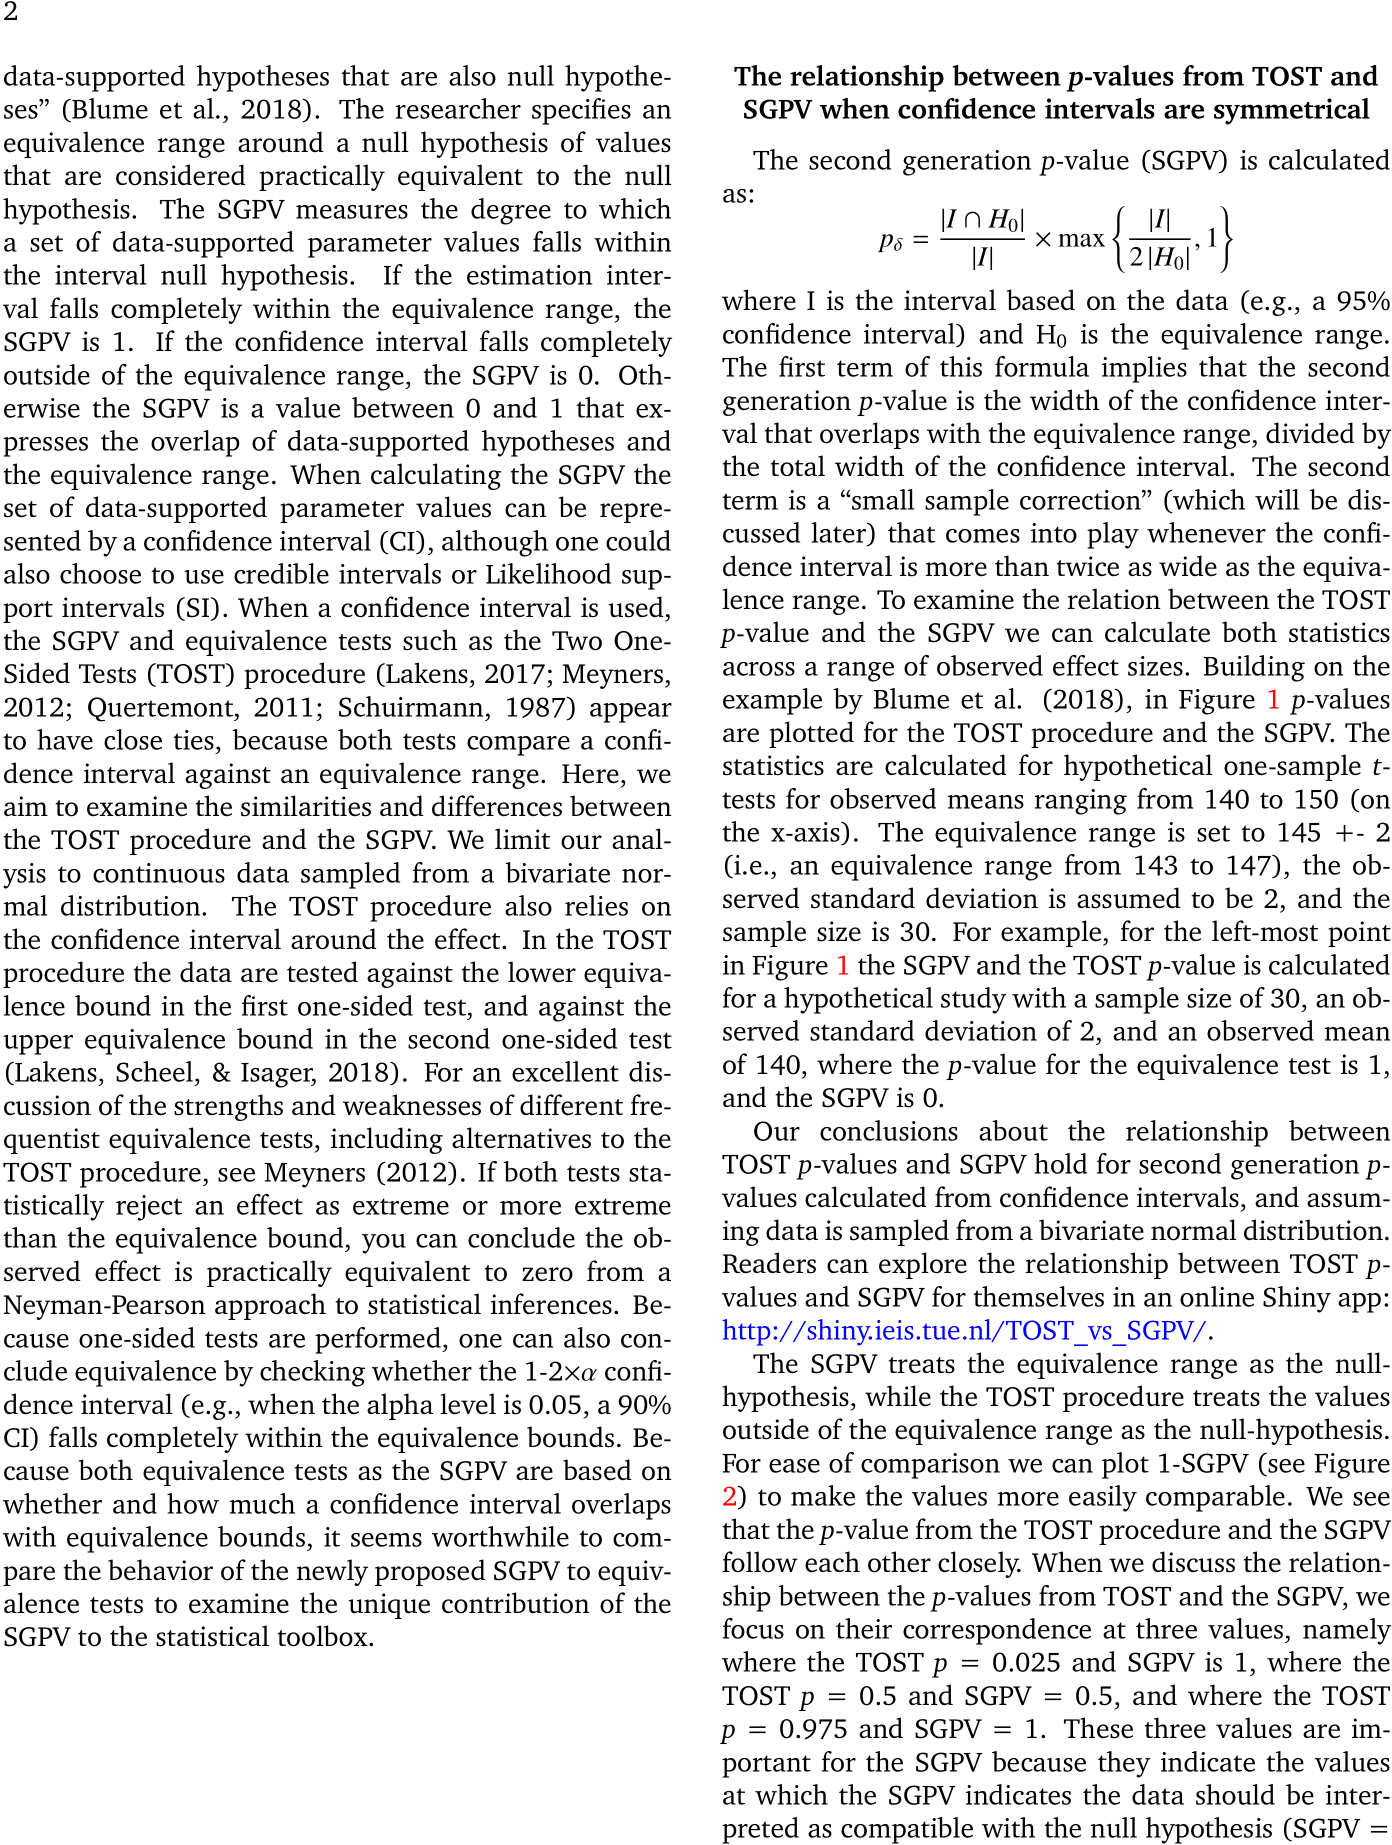
\includegraphics[width=5.51in]{C:/Users/Admin/OneDrive/Documents/Github projects/thesis/Chapitre 5/Chapitre 5-2} \end{center}

\begin{center}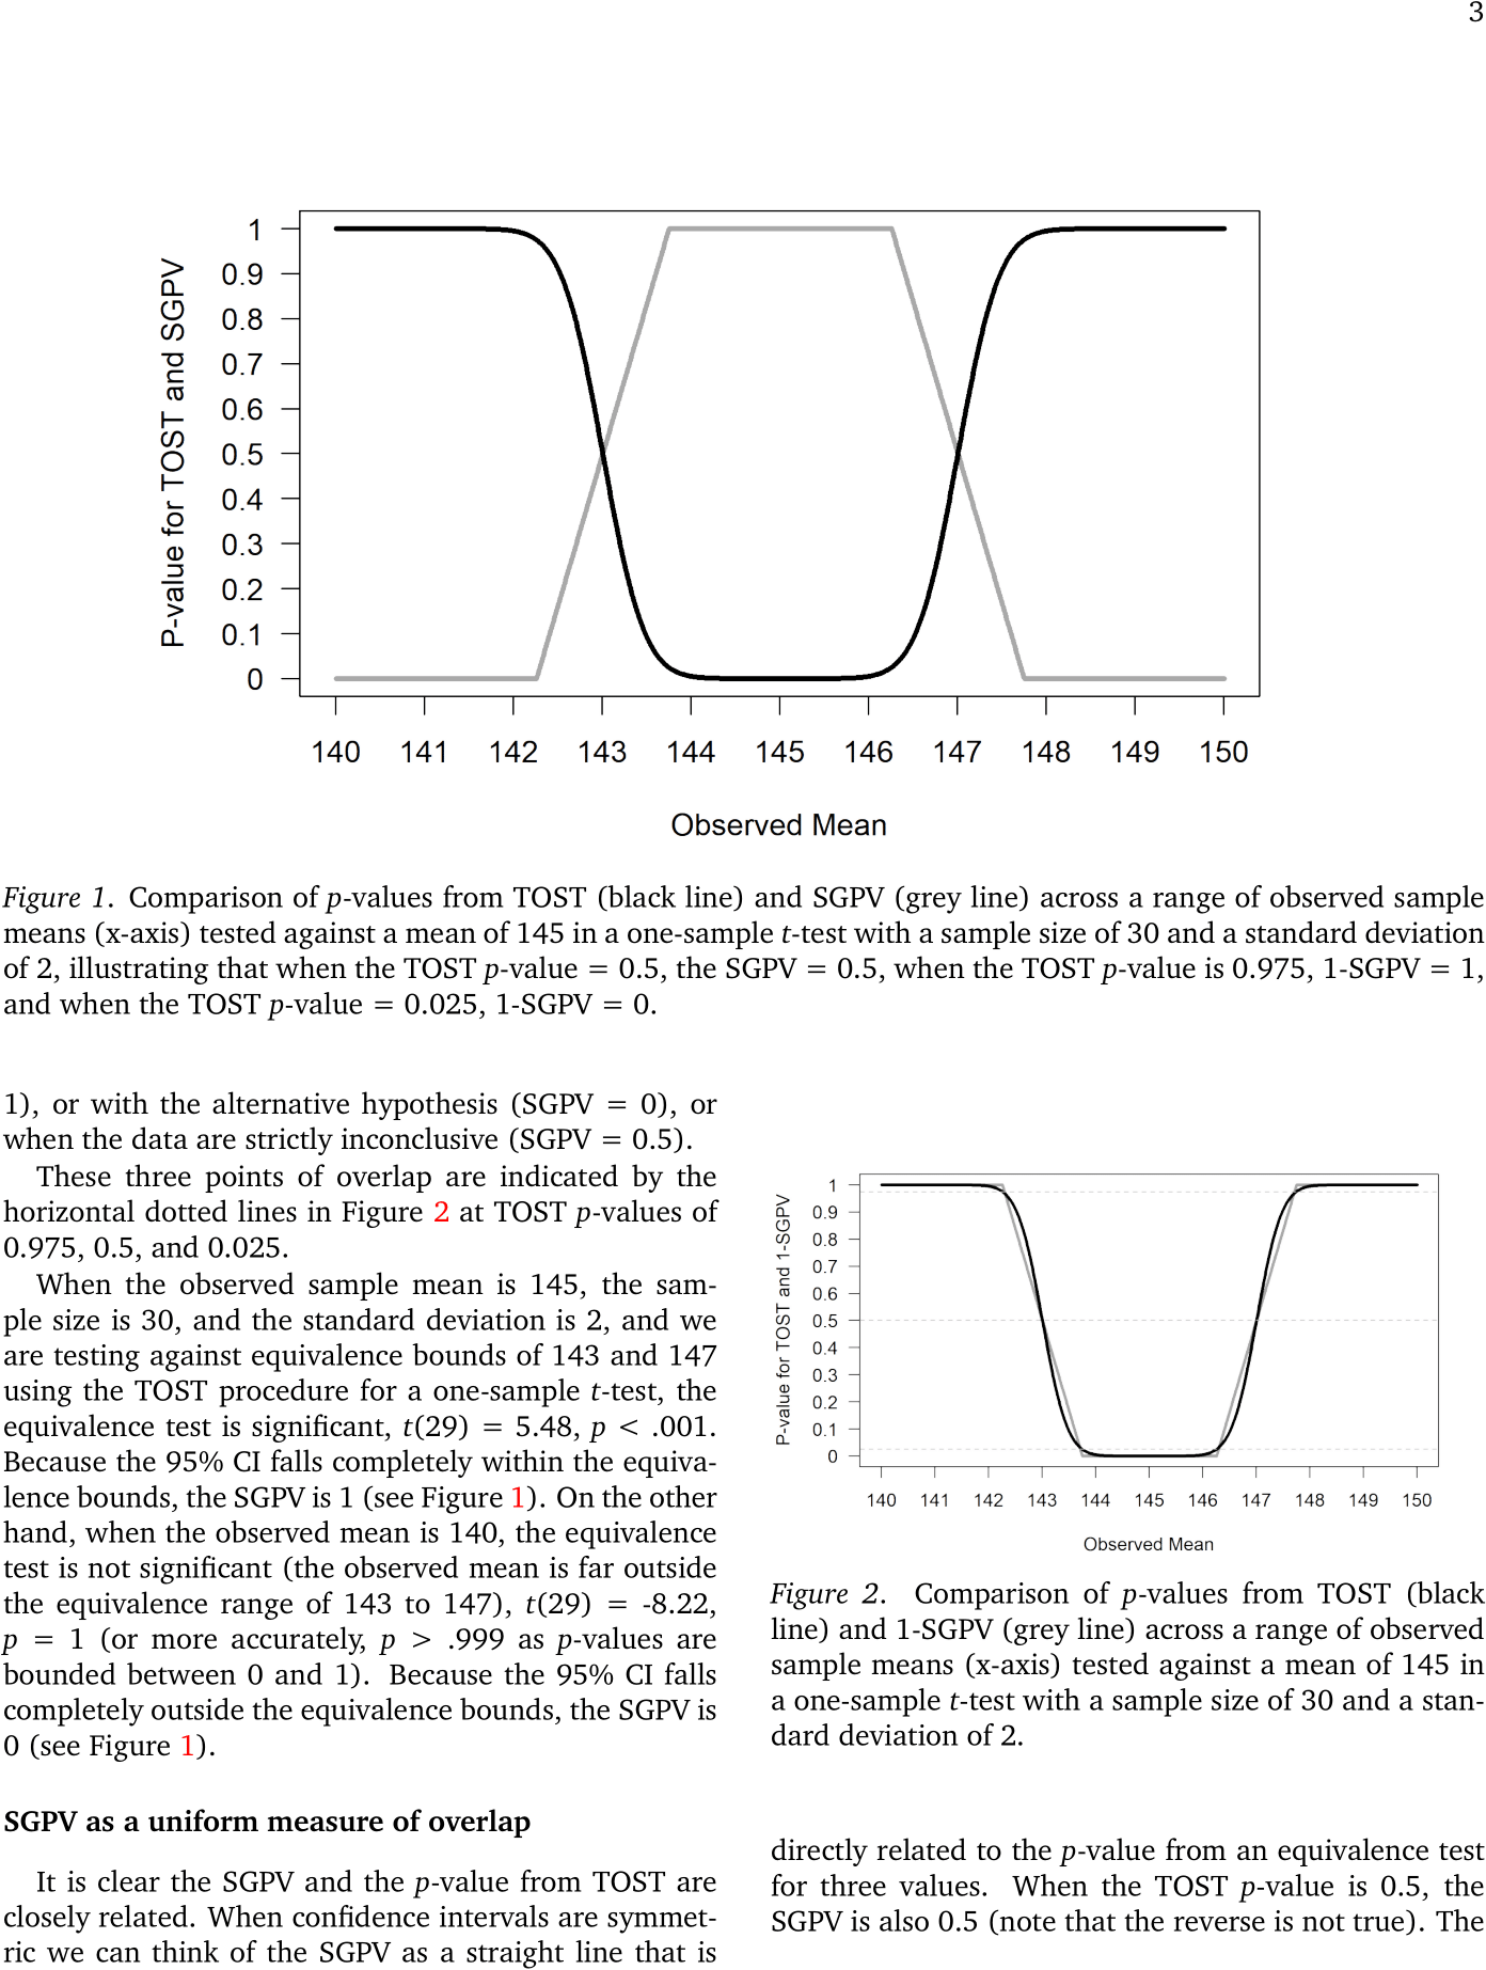
\includegraphics[width=5.51in]{C:/Users/Admin/OneDrive/Documents/Github projects/thesis/Chapitre 5/Chapitre 5-3} \end{center}

\begin{center}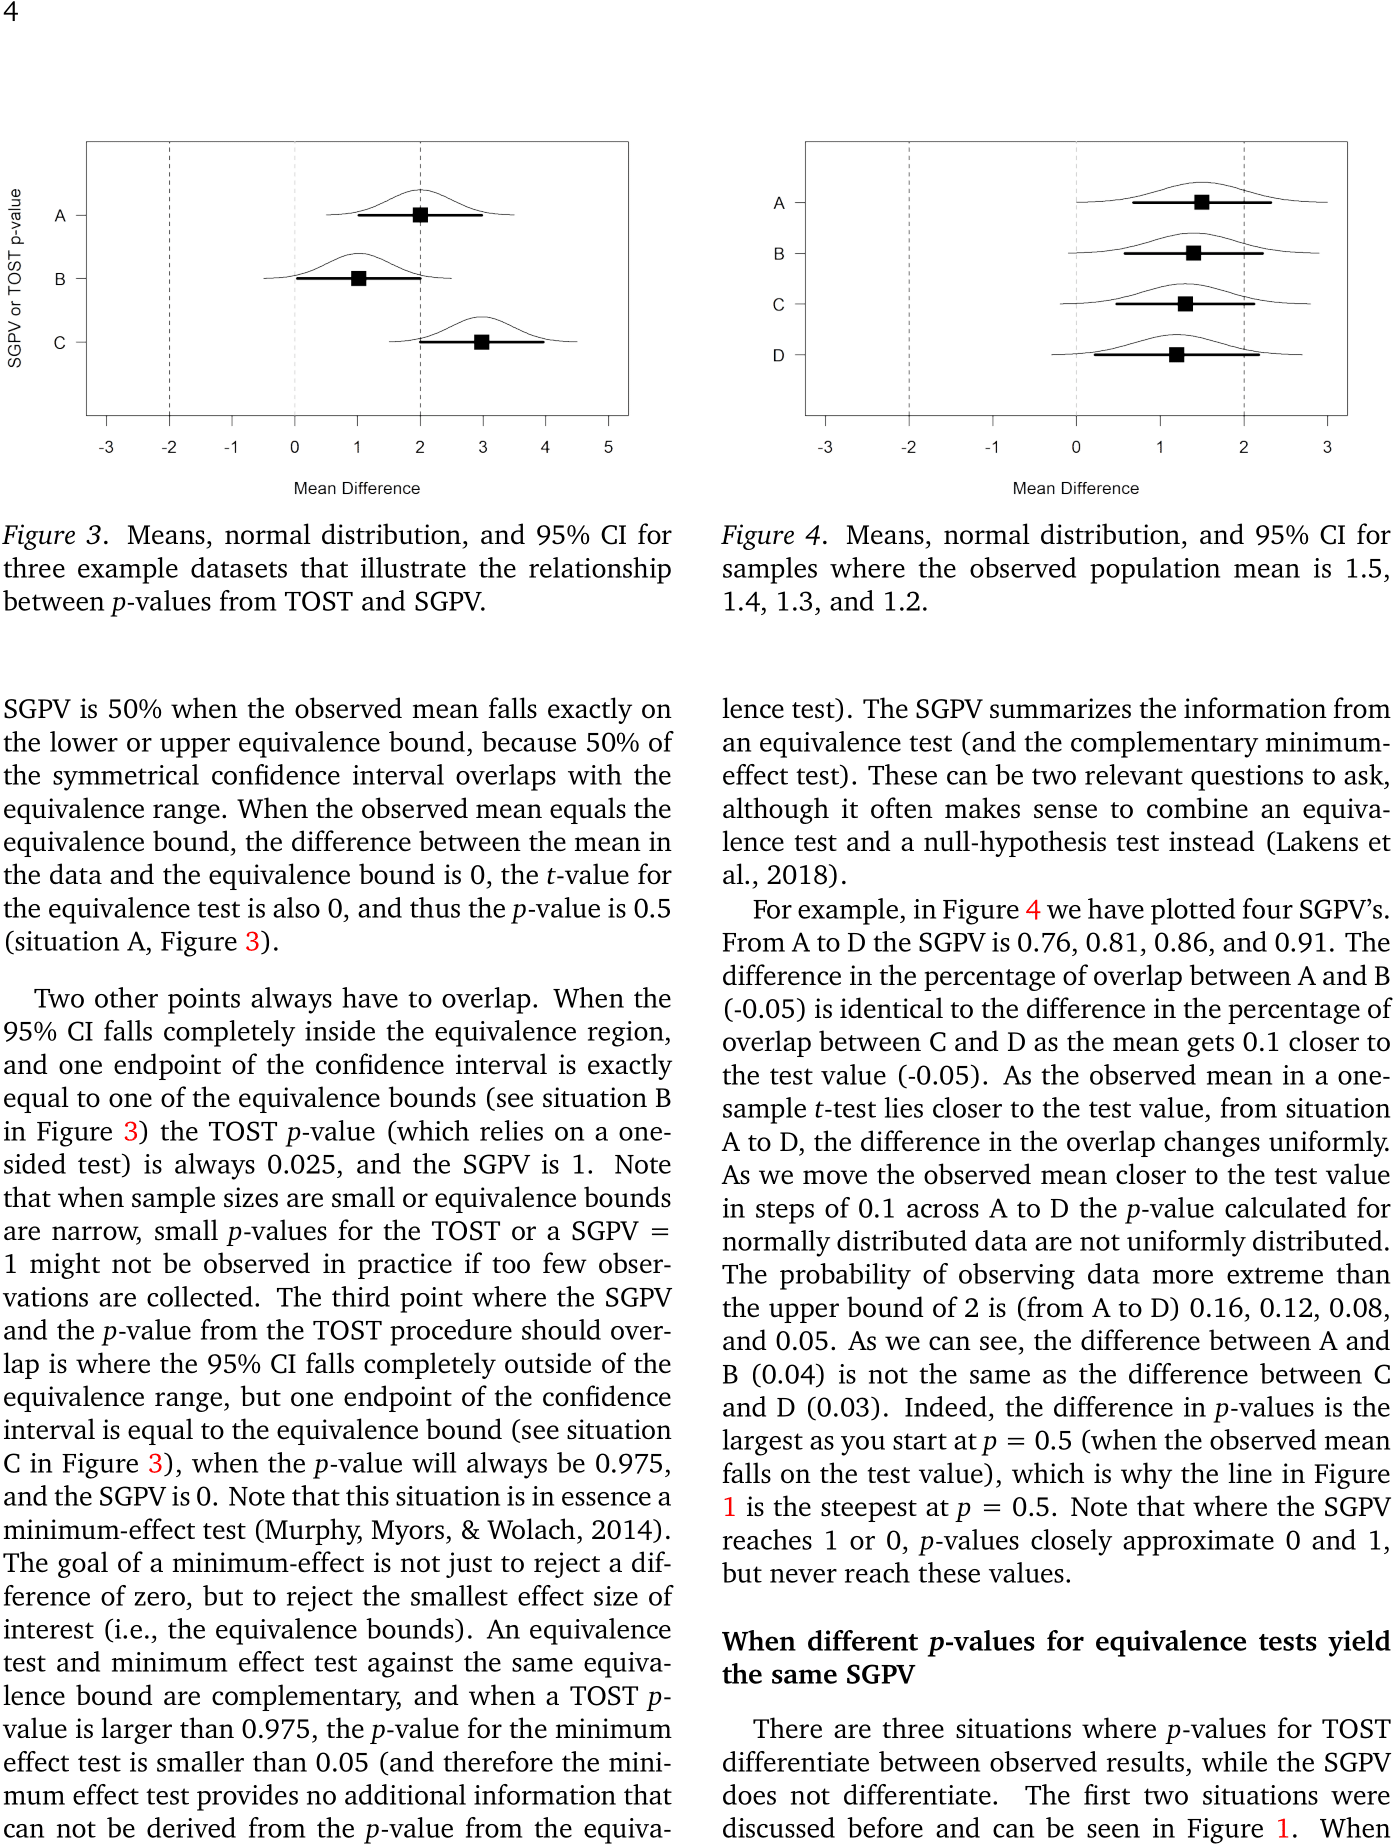
\includegraphics[width=5.51in]{C:/Users/Admin/OneDrive/Documents/Github projects/thesis/Chapitre 5/Chapitre 5-4} \end{center}

\begin{center}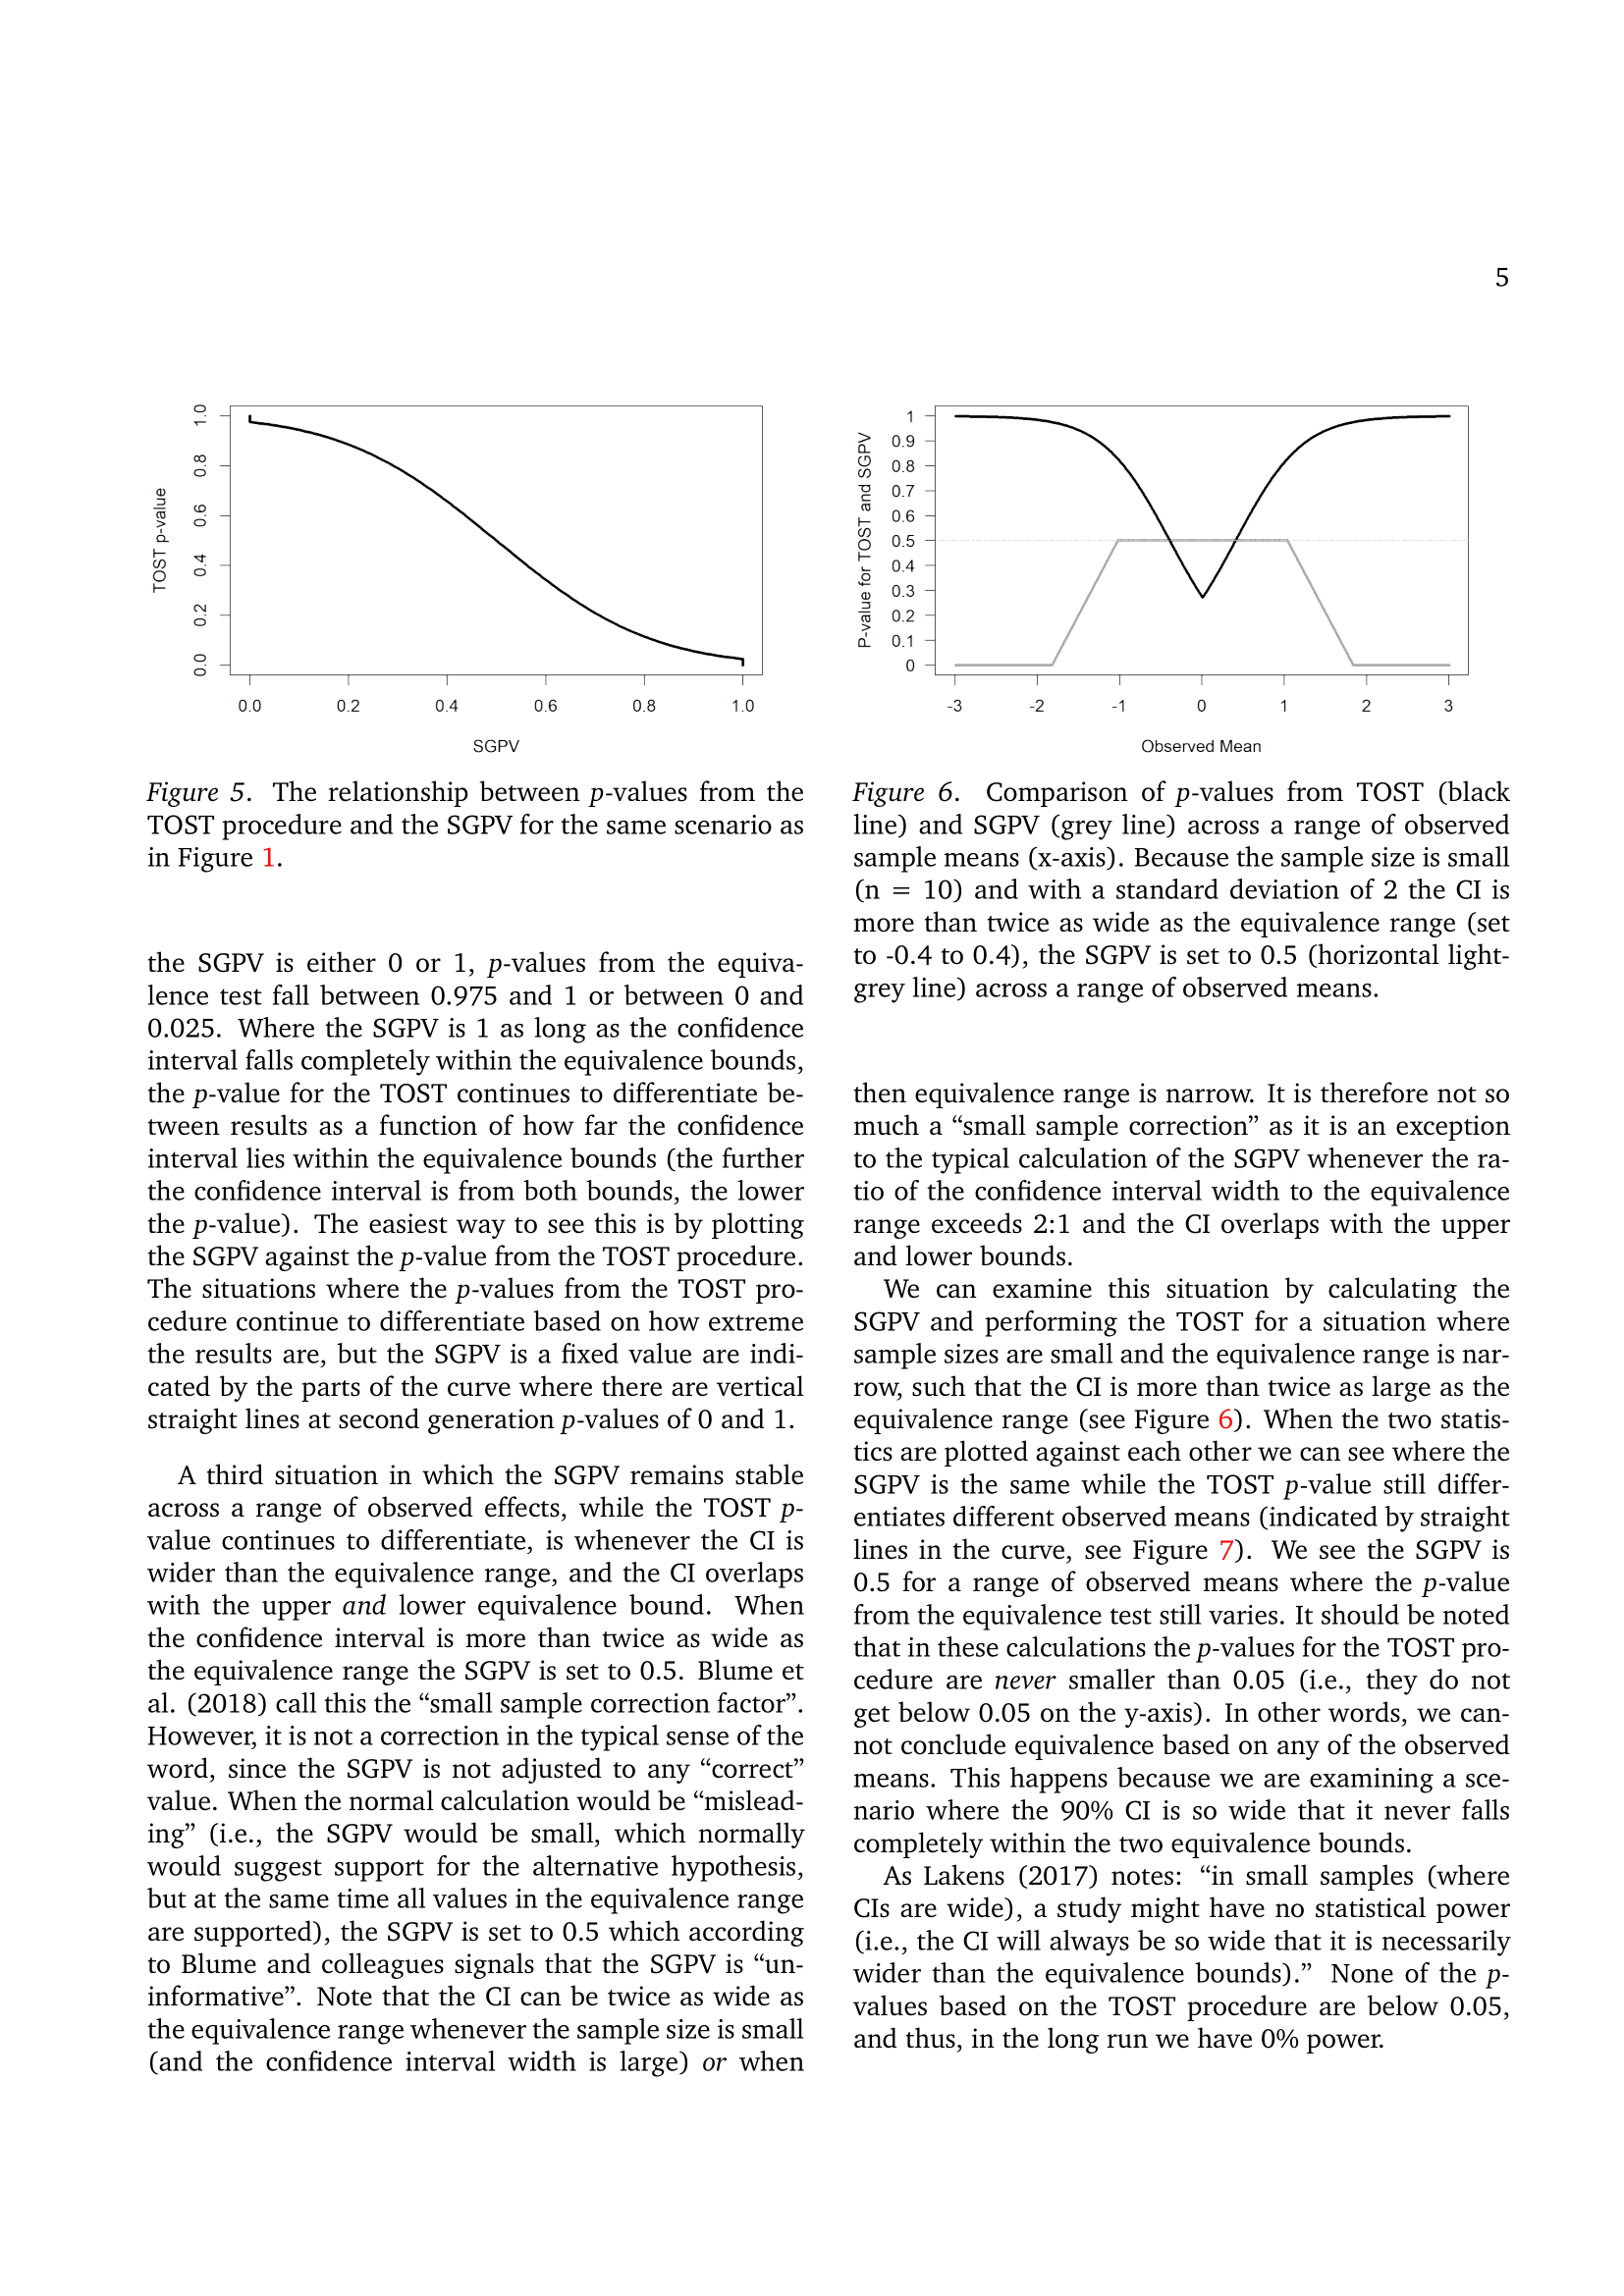
\includegraphics[width=5.51in]{C:/Users/Admin/OneDrive/Documents/Github projects/thesis/Chapitre 5/Chapitre 5-5} \end{center}

\begin{center}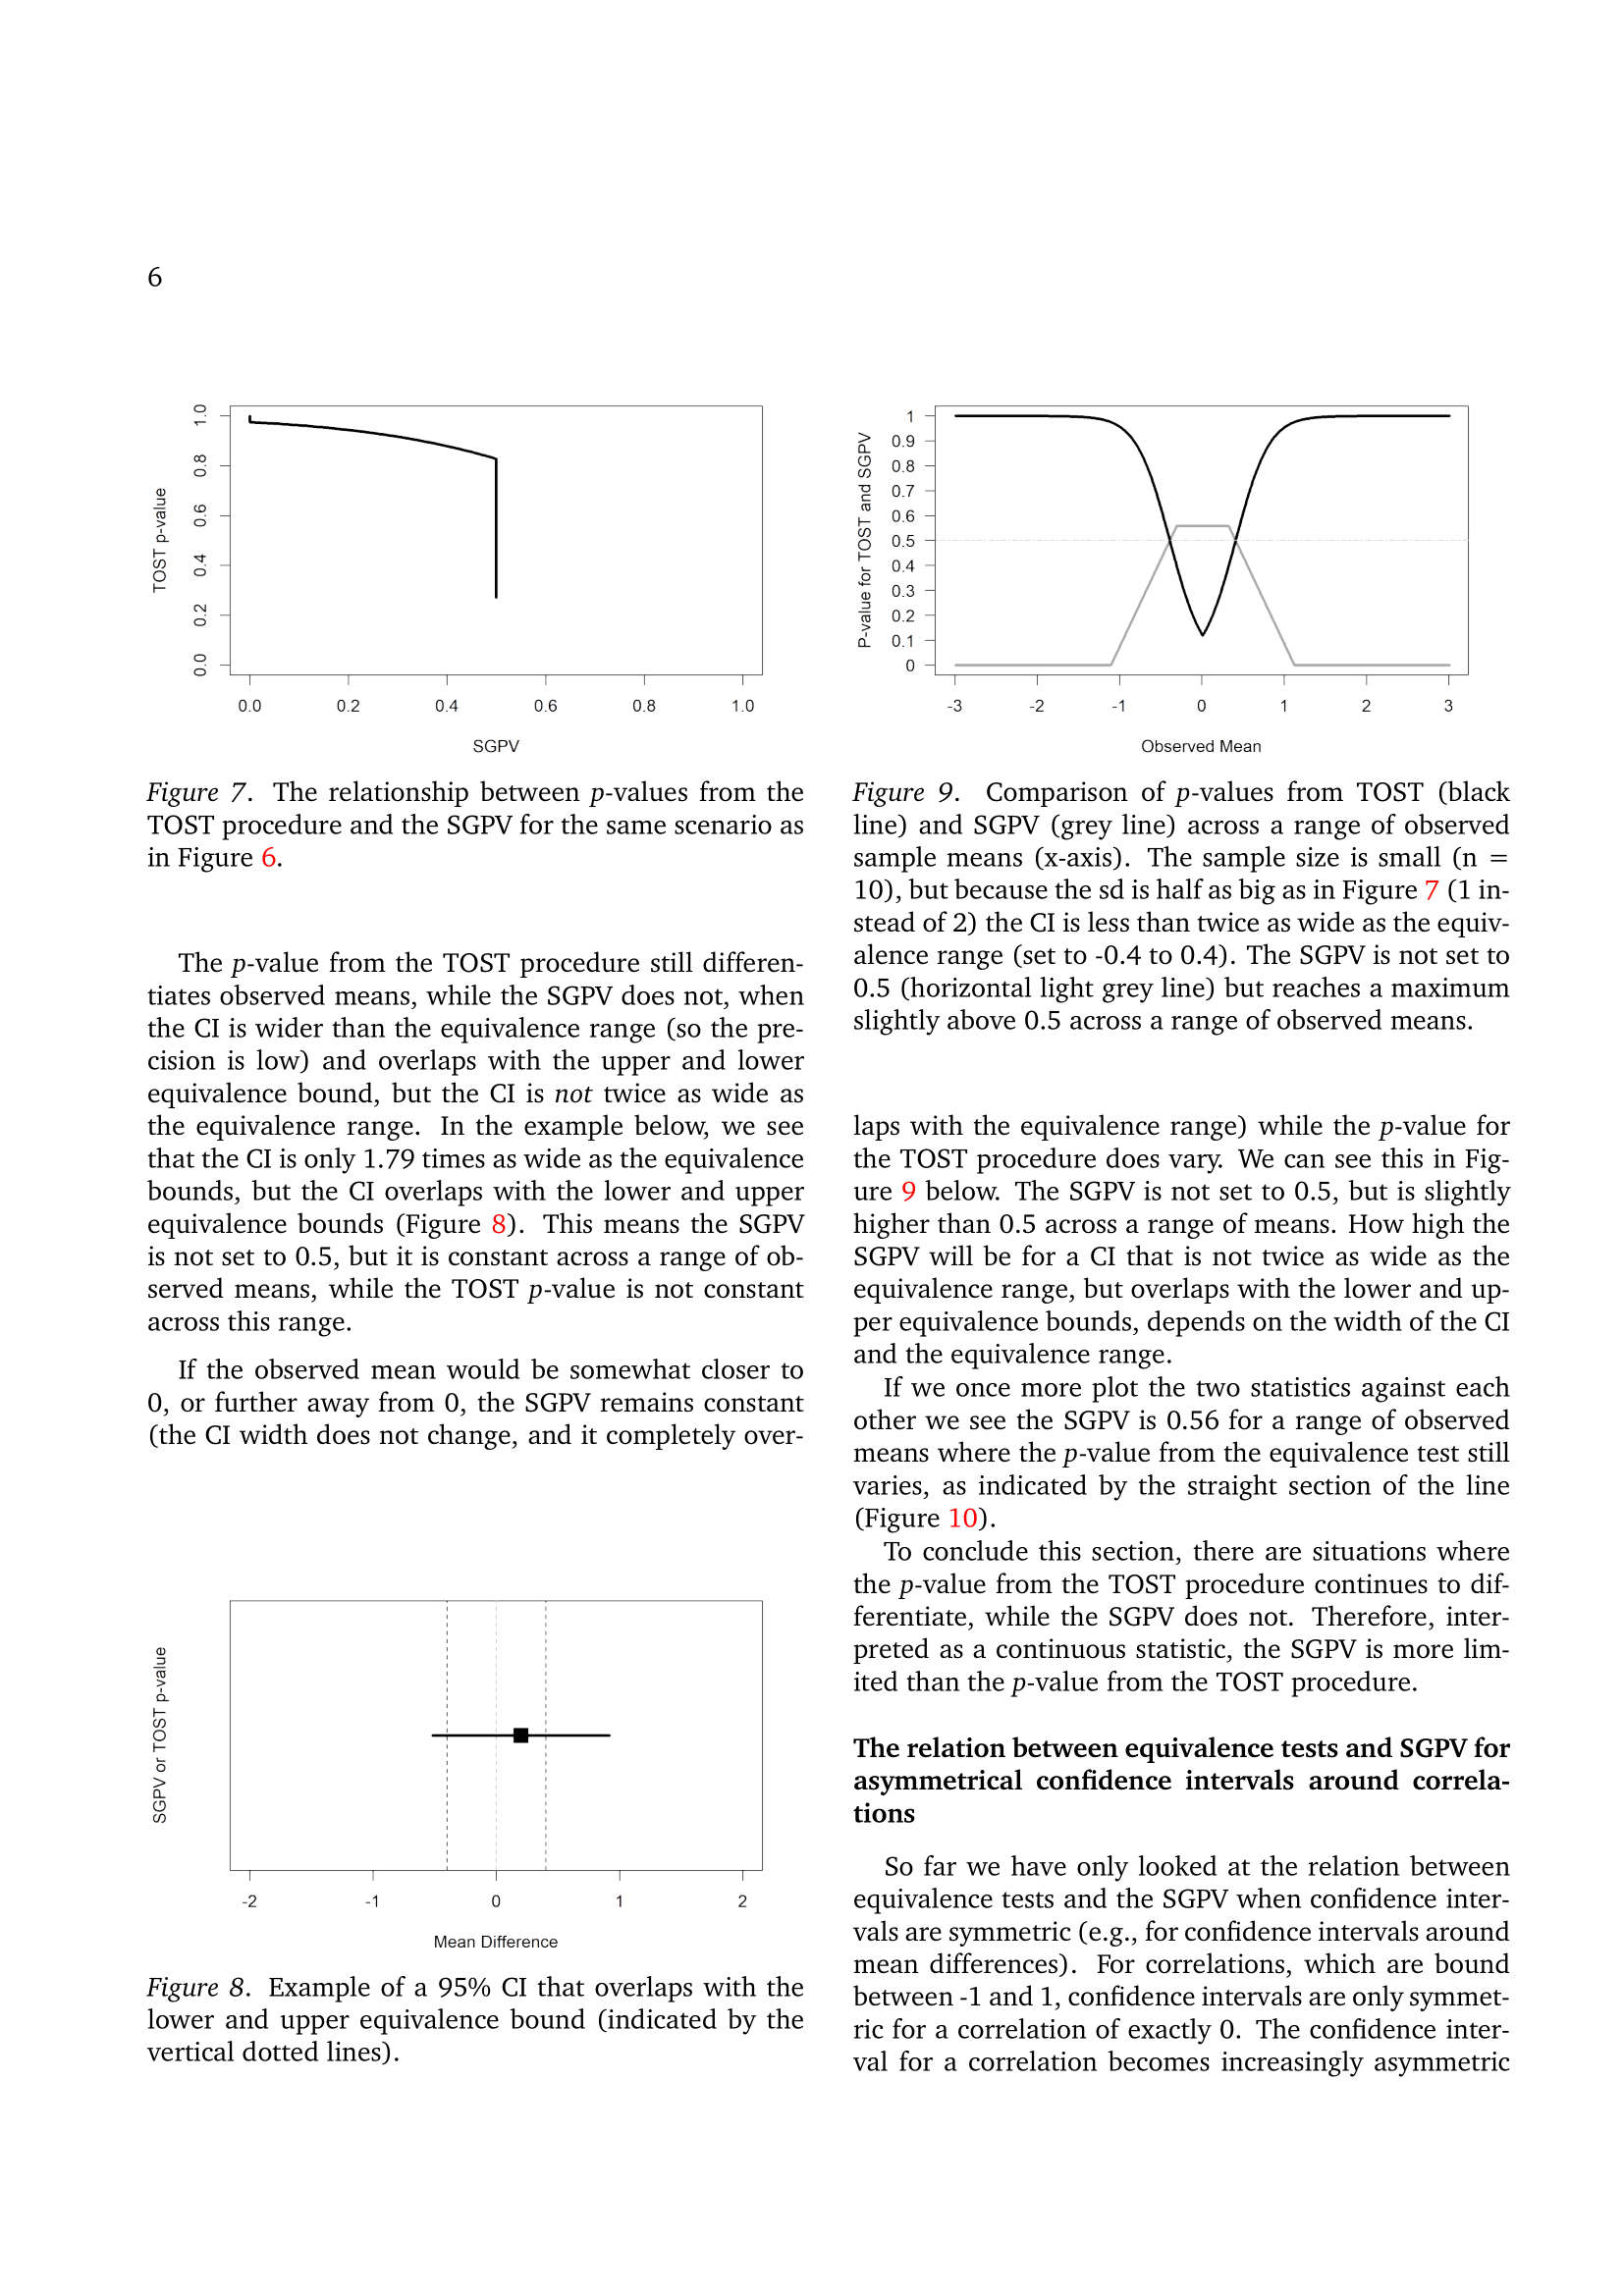
\includegraphics[width=5.51in]{C:/Users/Admin/OneDrive/Documents/Github projects/thesis/Chapitre 5/Chapitre 5-6} \end{center}

\begin{center}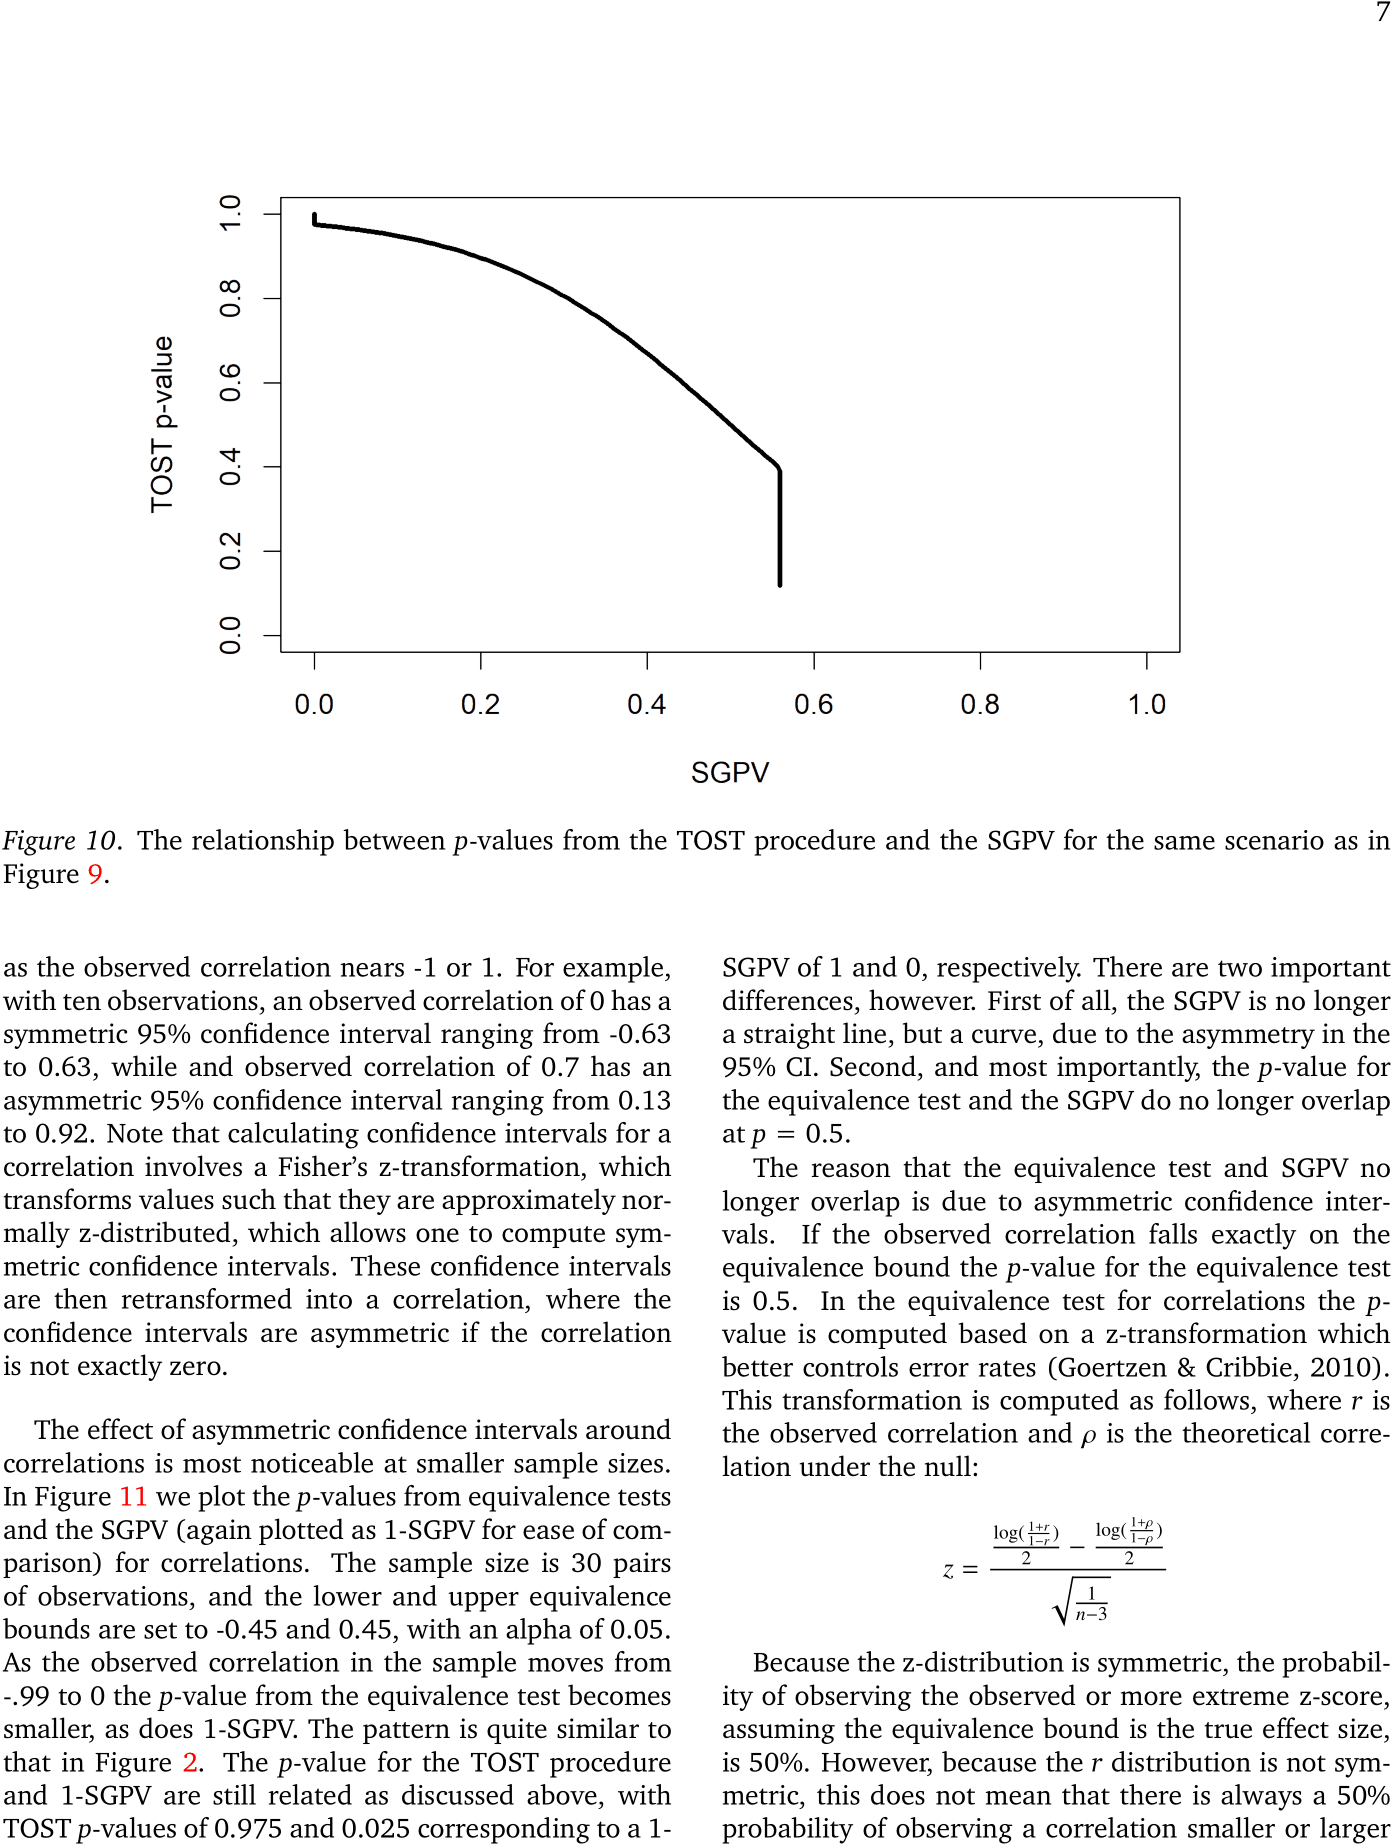
\includegraphics[width=5.51in]{C:/Users/Admin/OneDrive/Documents/Github projects/thesis/Chapitre 5/Chapitre 5-7} \end{center}

\begin{center}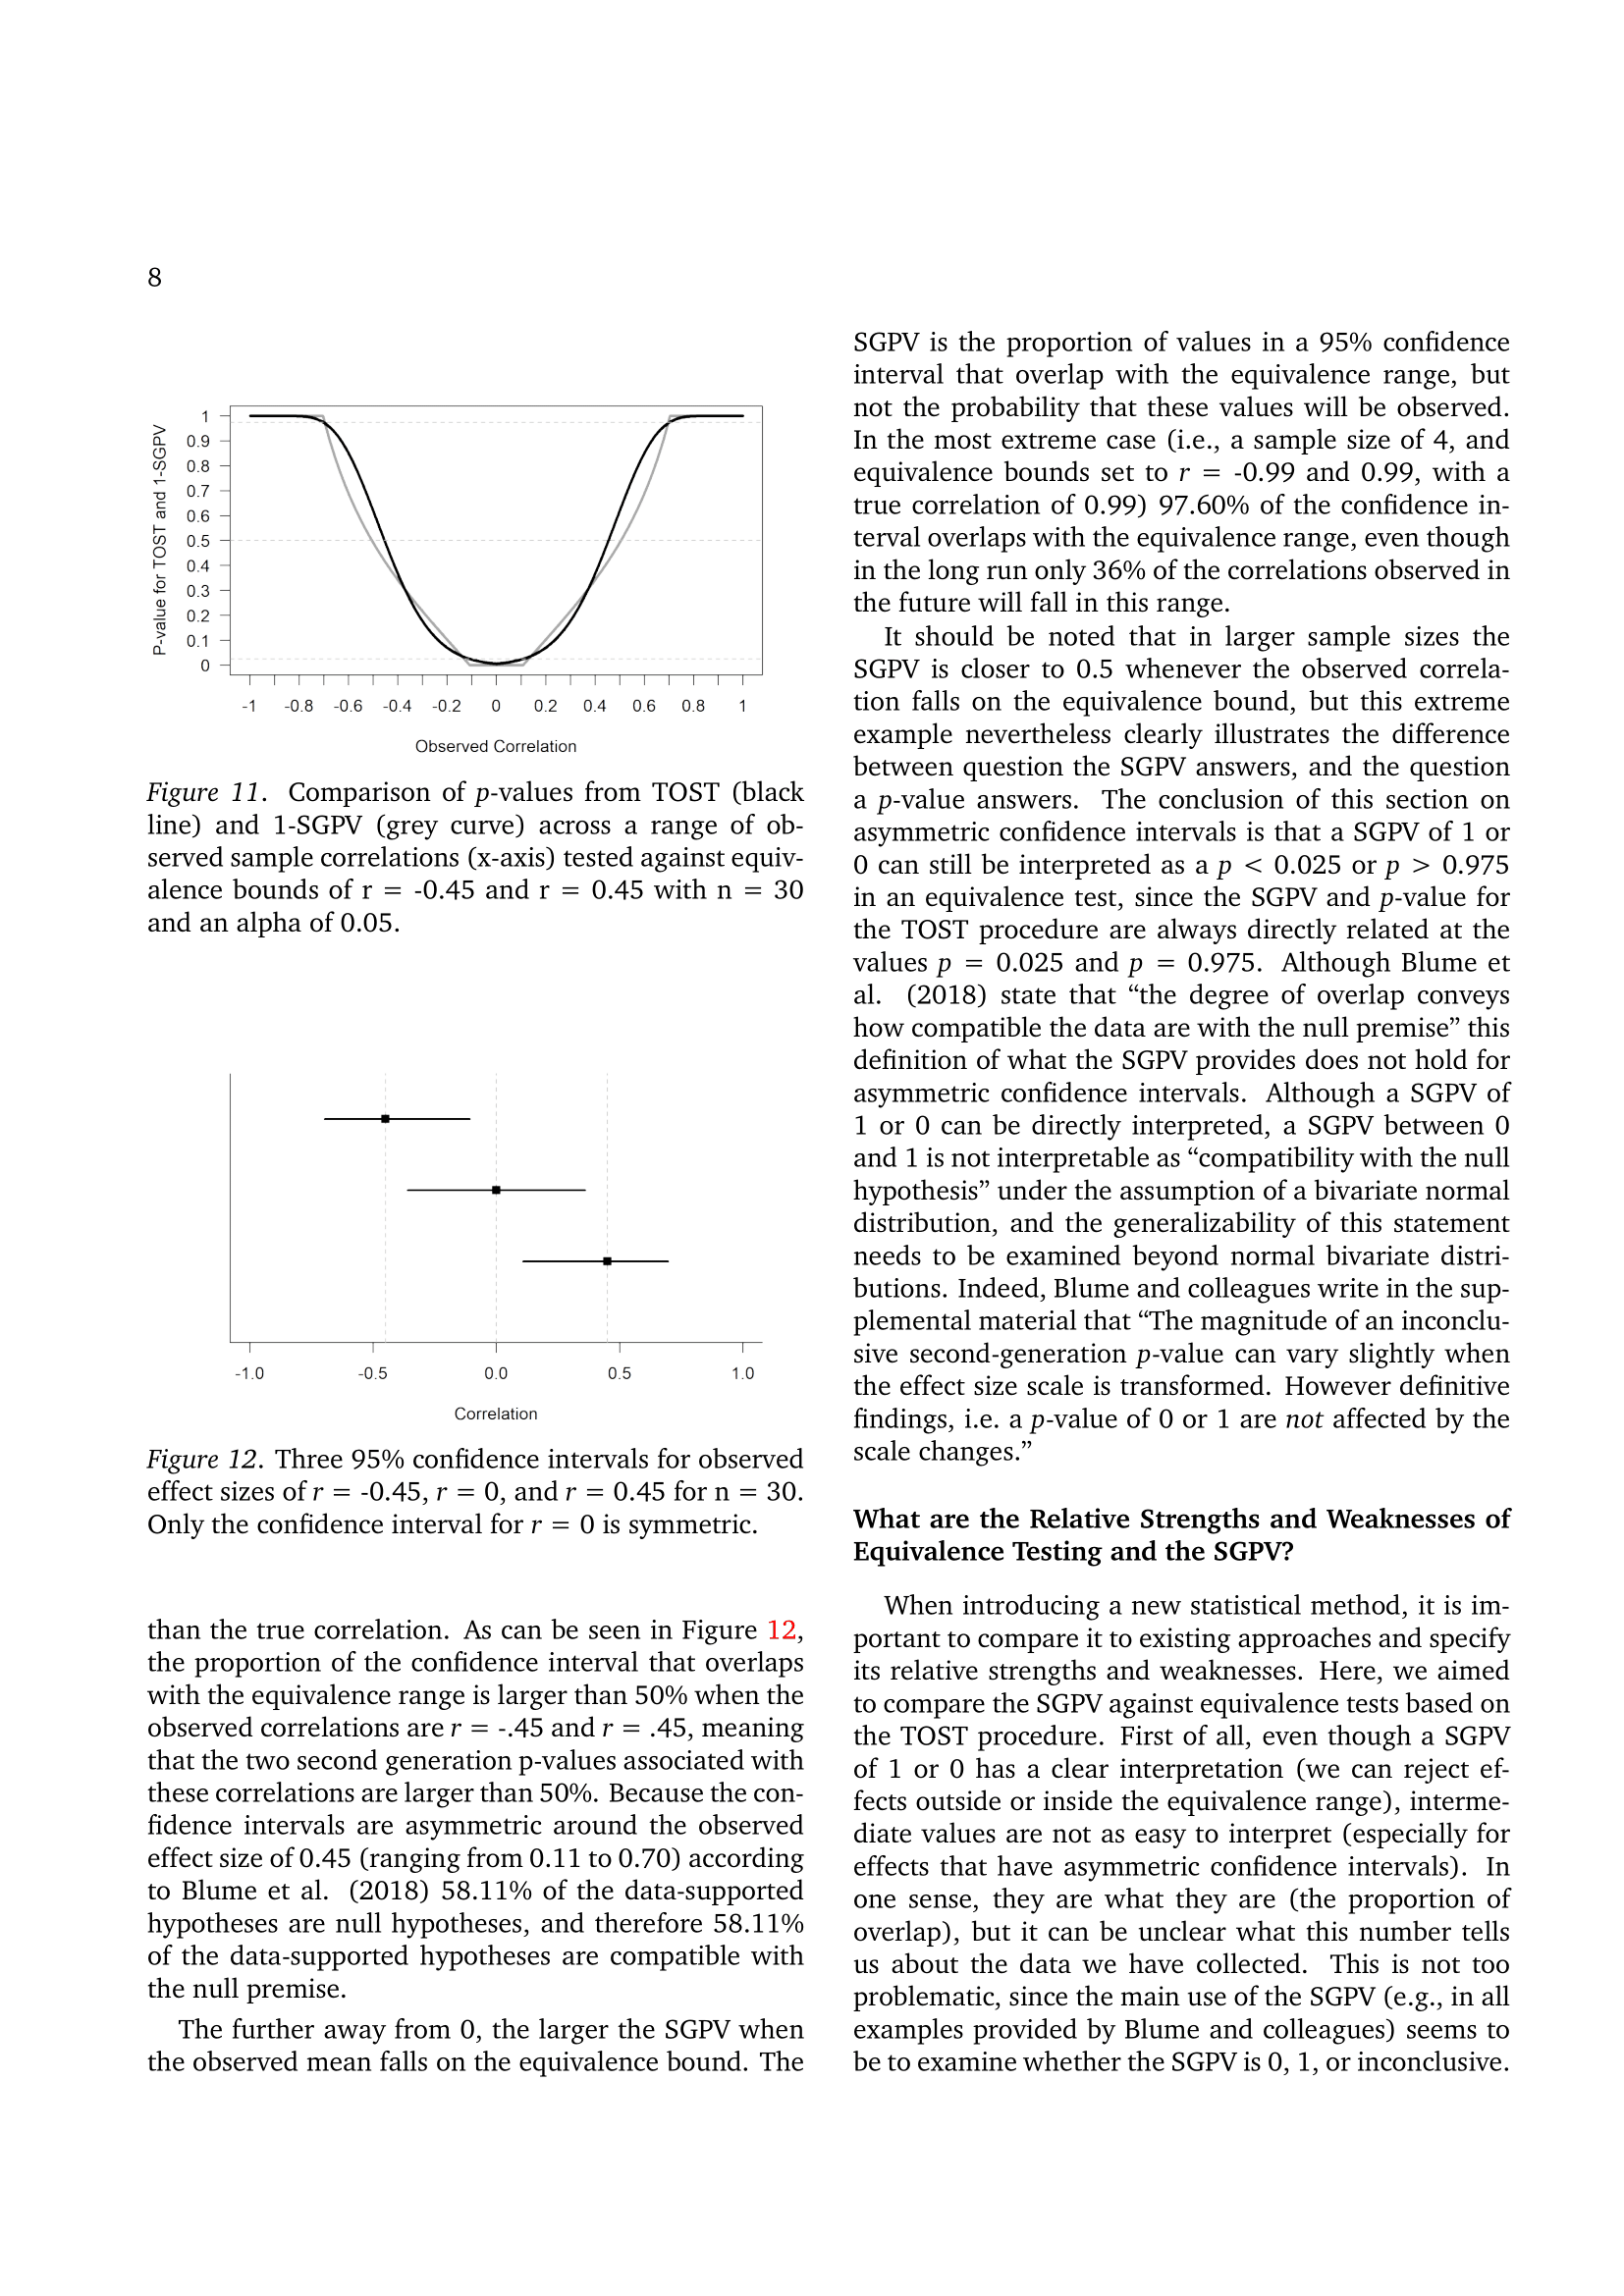
\includegraphics[width=5.51in]{C:/Users/Admin/OneDrive/Documents/Github projects/thesis/Chapitre 5/Chapitre 5-8} \end{center}

\begin{center}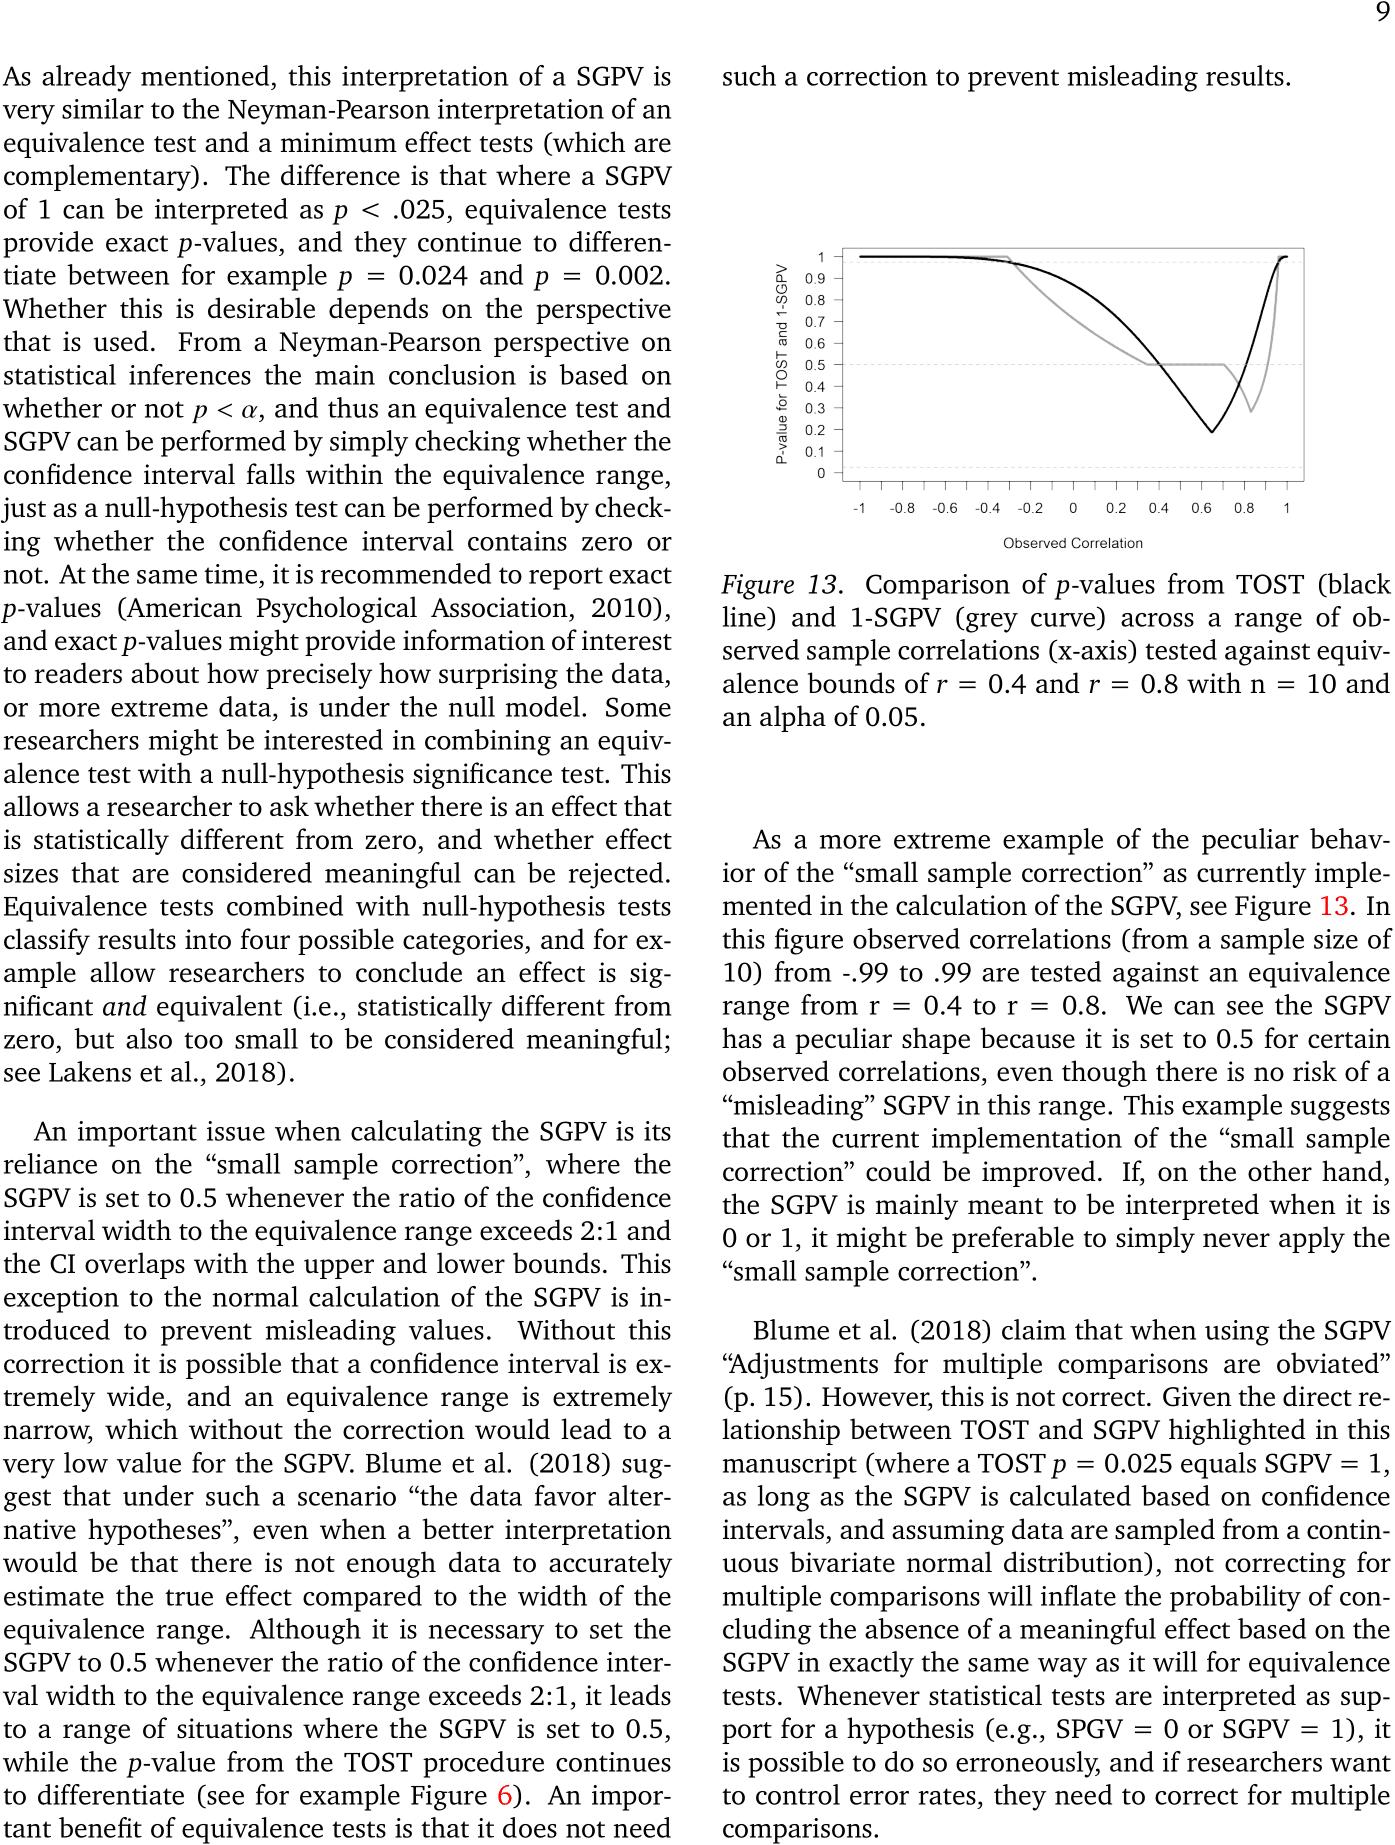
\includegraphics[width=5.51in]{C:/Users/Admin/OneDrive/Documents/Github projects/thesis/Chapitre 5/Chapitre 5-9} \end{center}

\begin{center}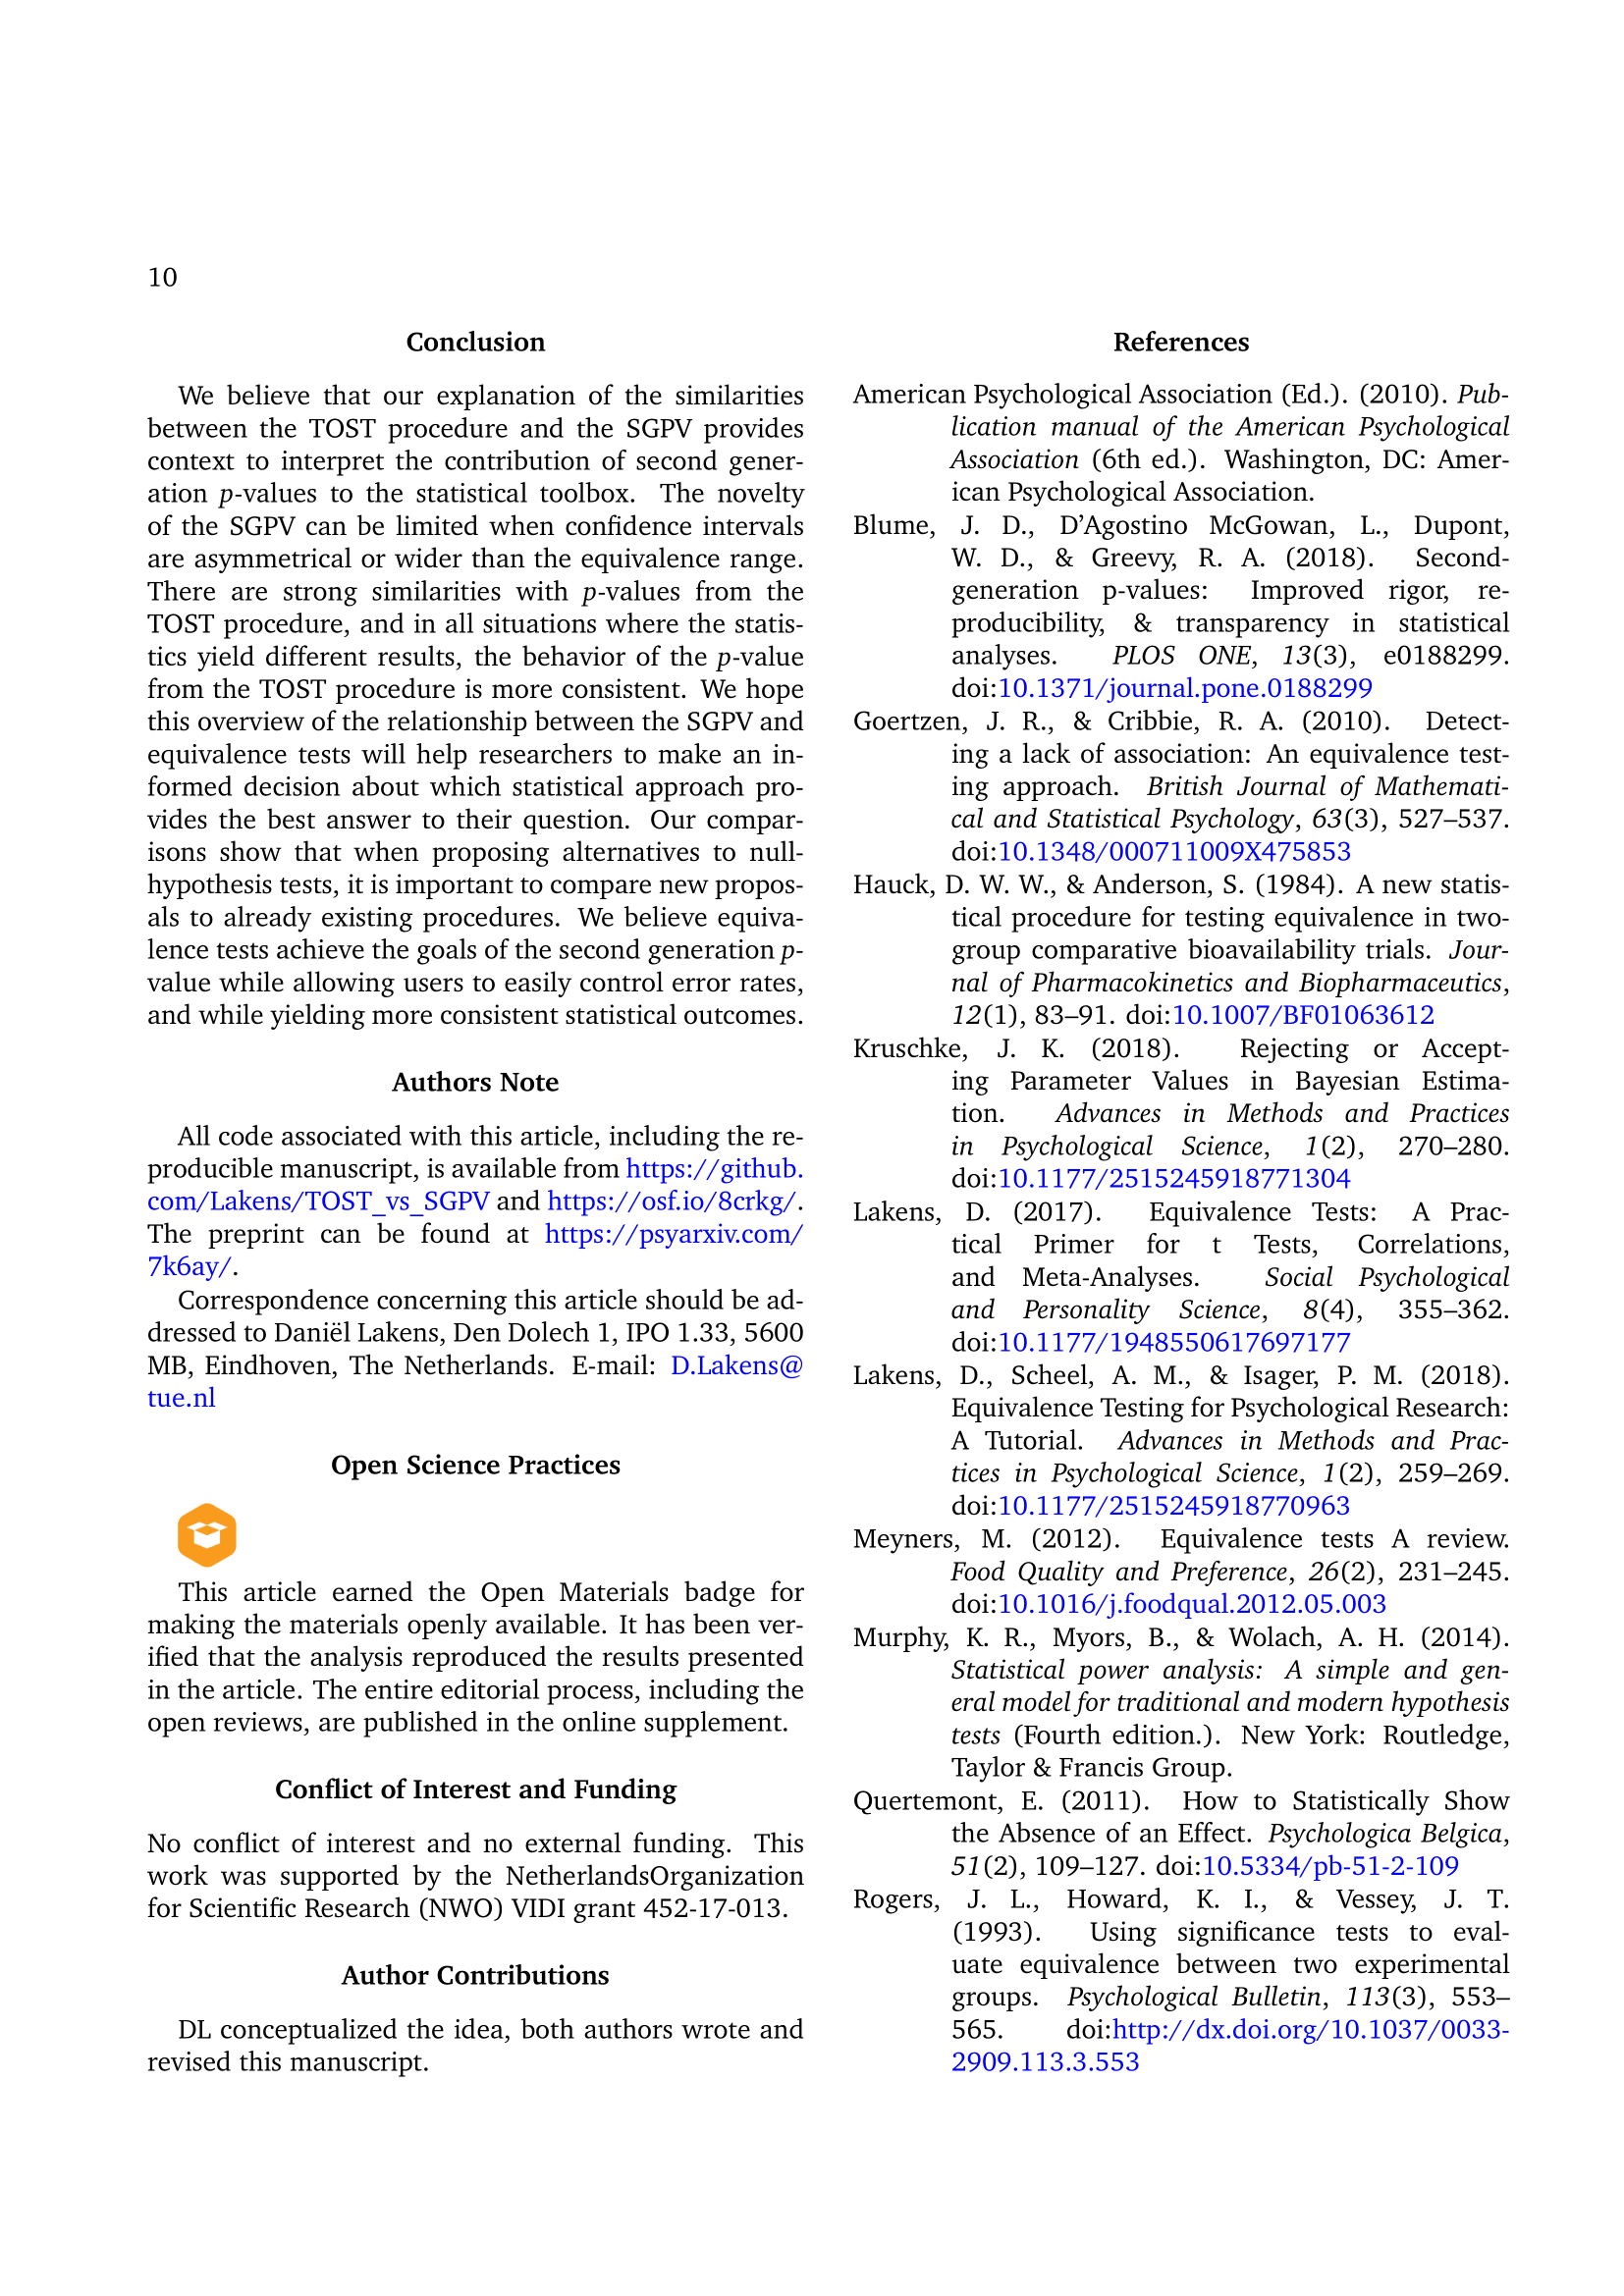
\includegraphics[width=5.51in]{C:/Users/Admin/OneDrive/Documents/Github projects/thesis/Chapitre 5/Chapitre 5-10} \end{center}

\begin{center}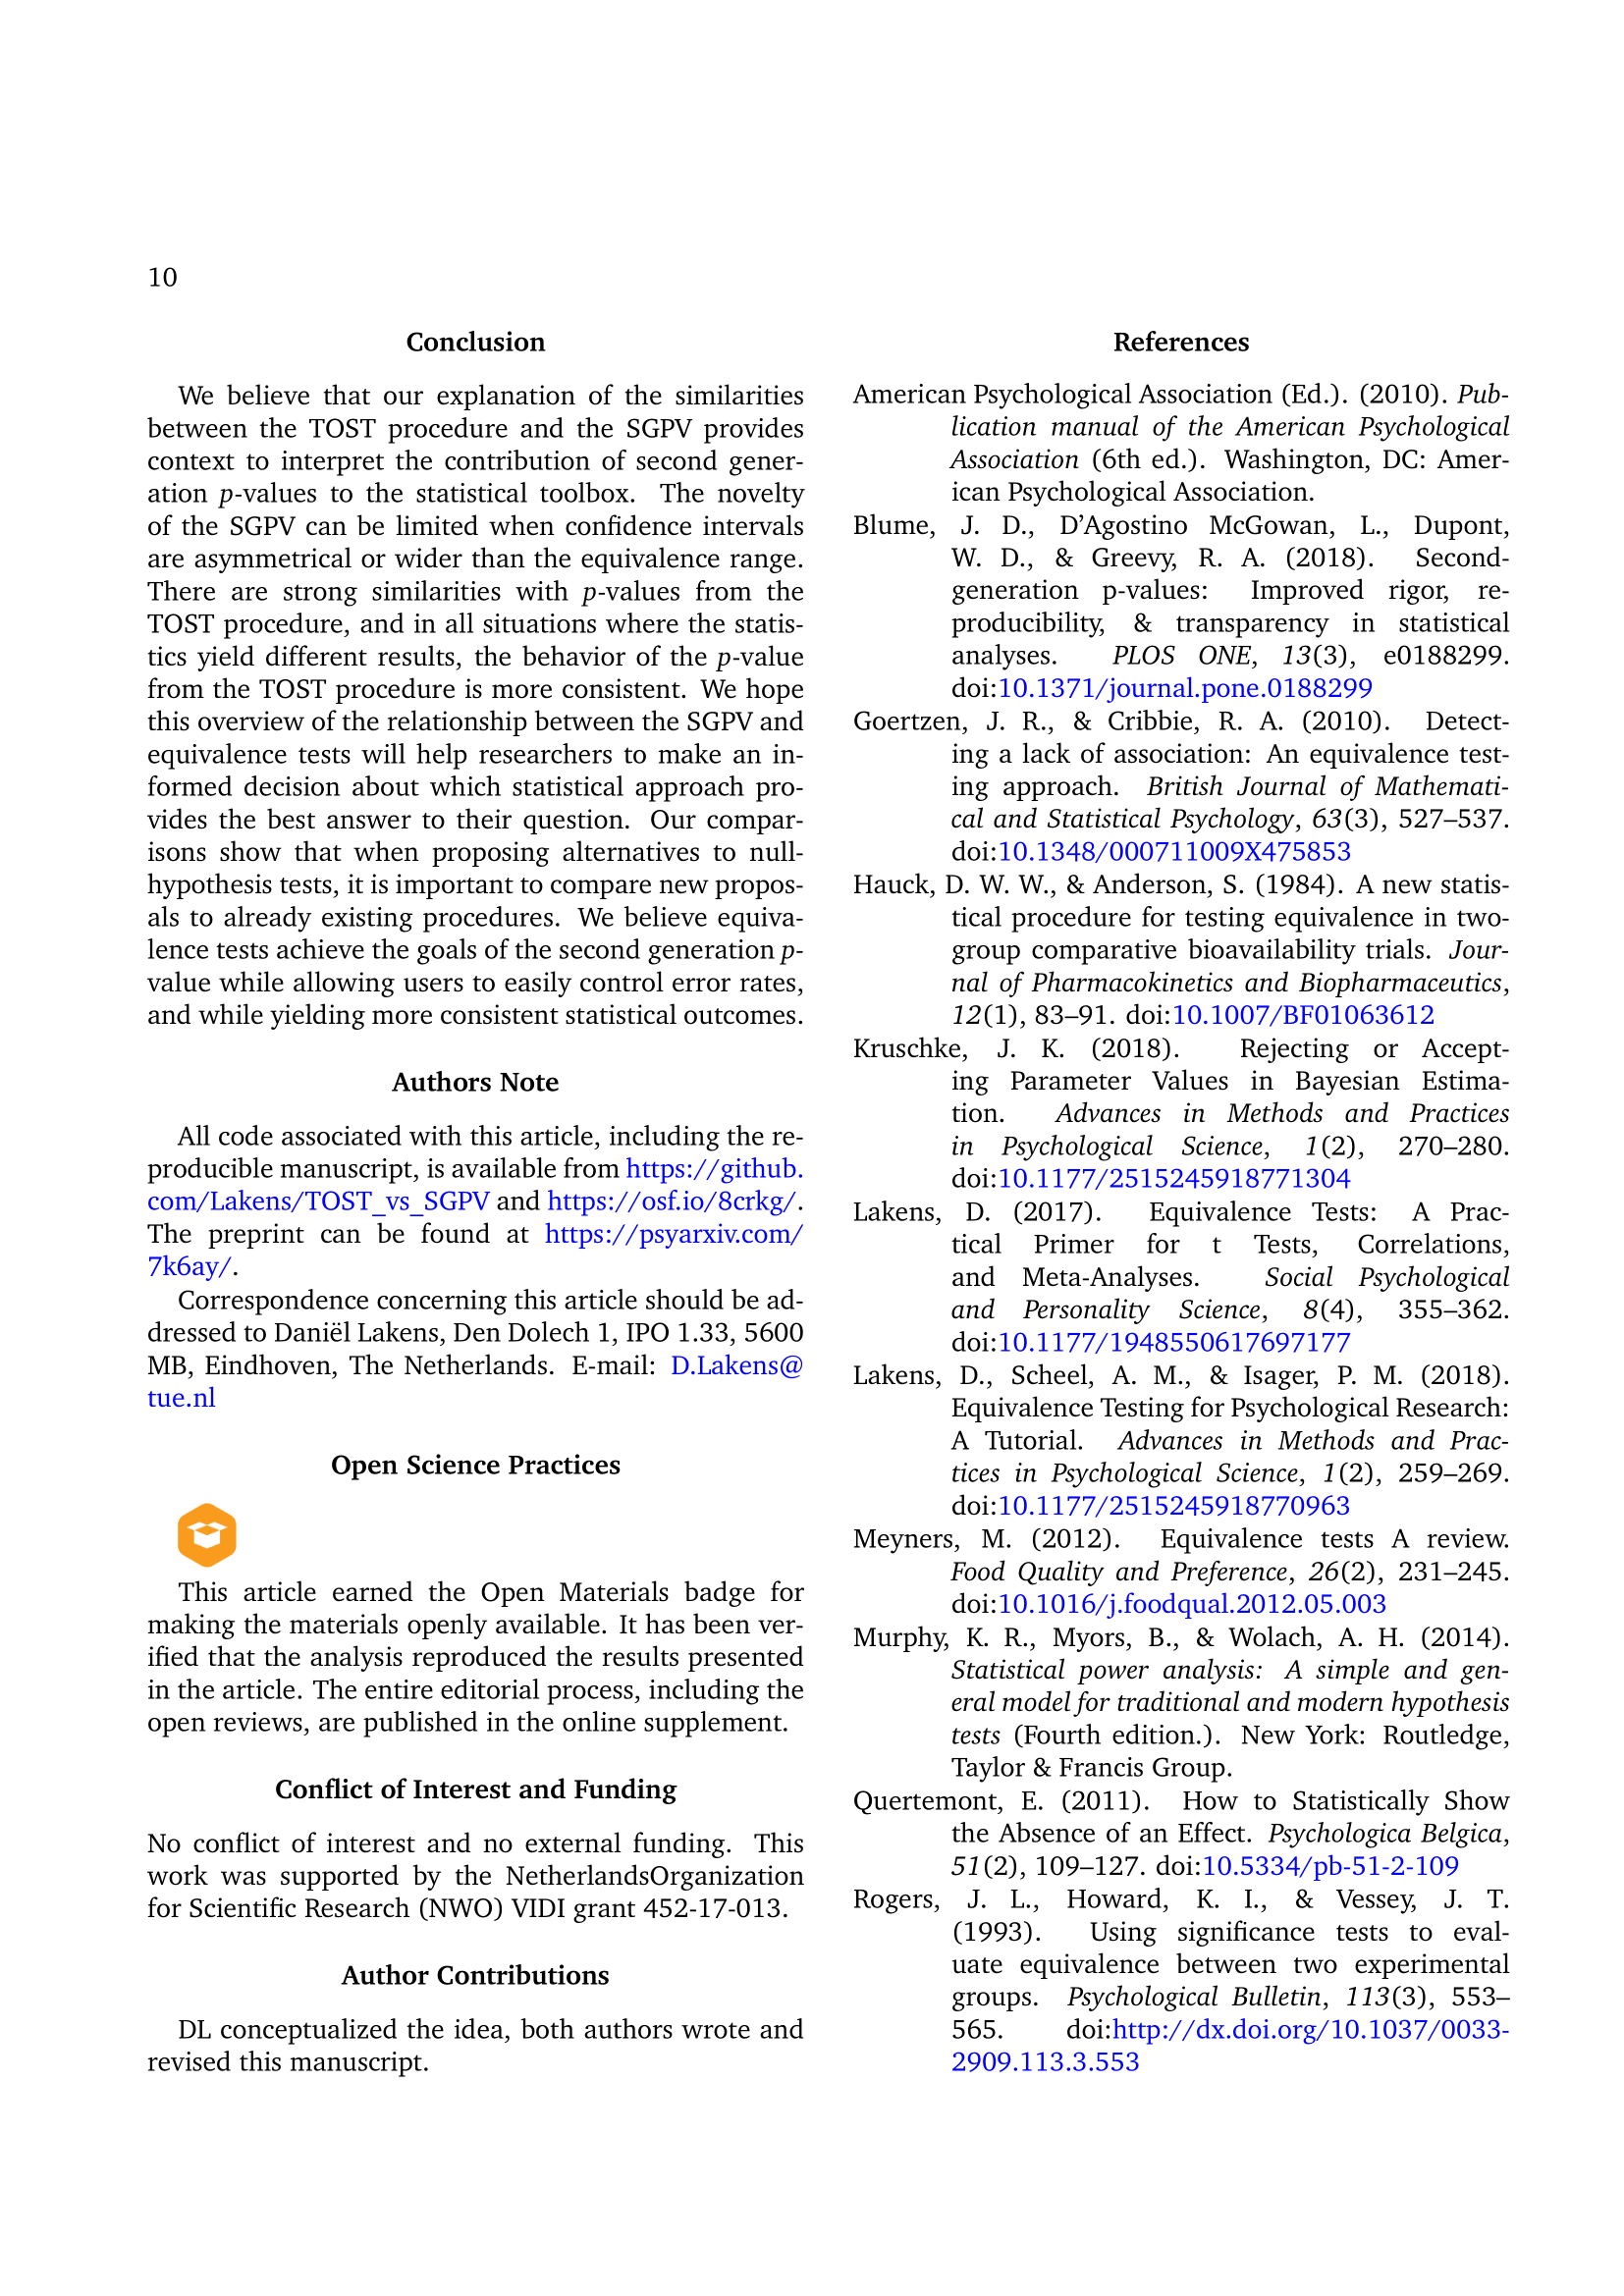
\includegraphics[width=5.51in]{C:/Users/Admin/OneDrive/Documents/Github projects/thesis/Chapitre 5/Chapitre 5-10} \end{center}


\end{document}
